\documentclass[openany]{book}
\usepackage[utf8]{inputenc}
\usepackage{verbatim}
%MODIFICAR

%%%%%%%%%%%%%%%%%%%%%%%

%%%%%%%%%%%%%%%%%%%%%%%
% HOLA PACO
% ESTE ES EL ARCHIVO DE LAS DEFINICIONES ESTRUCTURALES
% VERSION 1.1 NOMÁS
%
% AUTOR ORIGINAL:
% EDUARDO (CHITO) BELMONTE GUILLAMÓN
%
% ESTE ARCHIVO ES COMUNISTA, PUEDES COMPARTIRLO SI QUIERES
%%%%%%%%%%%%%%%%%%%%%%%

%----------------------------------
%     PAQUETICOS QUE SE USAN
%----------------------------------

%--------------------------
%    PARA USAR INKSCAPE
%---------------------------
\usepackage{import}
\usepackage{hyperref}
\usepackage{xifthen}
\usepackage{pdfpages}
\usepackage{transparent}

\newcommand{\incfig}[1]{%
    \def\svgwidth{\columnwidth}
    \import{./figures/}{#1.pdf_tex}
}

\newcommand{\custincfig}[2]{%
    \def\svgwidth{#1}
    \import{./figures/}{#2.pdf_tex}
}
\newcommand{\textnexttofig}[3]{
  \begin{minipage}[l]{0.45\textwidth}
    \custincfig{#1}{#2}
  \end{minipage}
  \begin{minipage}[l]{0.45\textwidth}
    #3
  \end{minipage}
}

%%%%%%%%% FIN DEL INKSCAPE

\usepackage{parskip} % Pa parrafos wapos
\setlength{\parindent}{0.5cm} % Pa la sangría
\usepackage{graphicx} % Pa meter las imágenes
\graphicspath{{Images/}} % La ruta a las imágenes

\usepackage{tikz} % Pa dibujar cosichuelas guapas

\usepackage[spanish]{babel} % PA QUE ESTÉ EN ESPAÑOL NOMÁS

\usepackage{enumitem} % Para personalizar las LISTAS YEAH

\setlist{nolistsep} % Pa que las listas estén junticas

\usepackage{booktabs} % Esta sirve para hacer tablas fancy con multicolumns y tal pero no tengo ni puta idea de usarla

\usepackage{xcolor} % PA DEFINIR LOS COLORINES
\definecolor{turquoise}{RGB}{21,103,112} % Es un turquesica así formal
\definecolor{violet}{RGB}{ 110, 6, 187 } % Color maricón

%-------------------------------------------------
%     MÁRGENES
%-------------------------------------------------

\usepackage{geometry}
\geometry{
    top=3cm,
    bottom=3cm,
    left=3cm,
    right=3cm,
    headheight=14pt,
	footskip=1.4cm,
	headsep=10pt,
}

\usepackage{avant} % Esto es una fuente para encabezados

%\usepackage{mathptmx} % Usar simbolitos matemáticos chulos

\usepackage{microtype} % Para fuentes de maricones

\usepackage[utf8]{inputenc} % Pa los acentos

\usepackage[T1]{fontenc}

%-------------------------------------------------
% Bibliografía e índice
%-------------------------------------------------

\usepackage{makeidx} % Pa hacer un índice
\makeindex

\usepackage{titletoc}   % Para manipular la tabla de contenidos

\contentsmargin{0cm}    % Para eliminar el margen por defecto

\usepackage{titlesec} % Pa cambiar los titulos skere

\titleformat
{\chapter} % command
[display] % shape
{\centering\bfseries\Huge\normalfont} % format
{\color{turquoise}  {\normalsize\MakeUppercase{Capítulo} \thechapter }} % label
{-0.5cm} % sep
{
    \color{turquoise}
    \rule{\textwidth}{3pt}
    \vspace{1ex}
    \centering
    \setcounter{ex}{0}
    \setcounter{dummy}{0}
} % before-code
[
\vspace{-0.5cm}%
\rule{\textwidth}{3pt}
] % after-code


\titleformat{\part}
[display]
{\centering\bfseries\Huge\normalfont}
{\color{turquoise} {\normalsize \MakeUppercase{Asignatura}}}
{0pt}
{\color{turquoise}
\vspace{-0.6cm}
\rule{\textwidth}{3pt}
\vspace{1ex}
\setcounter{chapter}{0}
\setcounter{section}{0}
\setcounter{dummy}{0}
\centering
}


\titleformat{\section}
{\normalfont\Large\bfseries}{\color{turquoise}\thesection\ - }{0.5em}{}

\usepackage{fancyhdr}   % Necesario para el encabezado y el pie de página

\pagestyle{fancy}   %Para modificar los encabezados
\fancyhf{}          %Para eliminar los encabezados y pies de página por defecto.
\fancyhead[LE,RO]{\sffamily\normalsize\thepage}
\fancyfoot[C]{Ampliación de Probabilidad}
%HACER

\usepackage{amsmath,amsfonts,amssymb,amsthm,cancel} % PARA LAS MATES

%   LINEA 199, HACER CAPULLADAS

\newtheoremstyle{turquoisebox}
{0pt} %Espacio encima
{0pt} %Espacio abajo
{\normalfont} % Fuente del cuerpo
{} % Cantidad de identado
{\small\ssfamily\color{turquoise}} % Fuente en la que pone "TEOREMA"
{:} % Puntuación tras el teorema
{0.25em} %Espacio tras el teorema
{\thmname{#1}\thmnumber{#2}} %No sé si esto funciona


\newcounter{dummy}
\newcounter{ex}
\newtheorem{teoremote}[dummy]{\color{turquoise}Teorema}
\newtheorem{propositiont}{\color{turquoise}Proposición}[section]
\newtheorem{lemmat}{\color{turquoise}Lema}[section]
\newtheorem{definitionT}{\color{turquoise}Definición}[section]
\newtheorem{exerciseT}[ex]{Ejercicio}
\newtheorem{examplote}[ex]{\color{turquoise}Ejemplo}
\newtheorem{methodT}[dummy]{\color{turquoise}Método}


\RequirePackage[framemethod=default]{mdframed} % Required for creating the theorem, definition, exercise and corollary boxes

%Caja de teoremas

\newmdenv[skipabove=7pt,
skipbelow=7pt,
backgroundcolor=black!5,
linecolor=turquoise,
innerleftmargin=5pt,
innerrightmargin=5pt,
innertopmargin=5pt,
leftmargin=0cm,
rightmargin=0cm,
linewidth=3pt,
innerbottommargin=5pt]{tBox}

\newmdenv[skipabove=7pt,
skipbelow=7pt,
backgroundcolor=black!5,
linecolor=turquoise,
innerleftmargin=5pt,
innerrightmargin=5pt,
innertopmargin=5pt,
leftmargin=0cm,
rightmargin=0cm,
linewidth=1pt,
innerbottommargin=5pt]{pBox}

\newmdenv[skipabove=7pt,
skipbelow=7pt,
backgroundcolor=violet!7,
linecolor=turquoise,
innerleftmargin=5pt,
innerrightmargin=5pt,
innertopmargin=5pt,
leftmargin=0cm,
rightmargin=0cm,
rightline=false,
topline=false,
bottomline=false,
linewidth=4pt,
innerbottommargin=5pt]{mBox}

\newmdenv[skipabove=7pt,
skipbelow=7pt,
rightline=false,
leftline=true,
topline=false,
bottomline=false,
linecolor=turquoise,
innerleftmargin=5pt,
innerrightmargin=5pt,
innertopmargin=0pt,
leftmargin=0cm,
rightmargin=0cm,
linewidth=4pt,
innerbottommargin=0pt]{dBox}

\newmdenv[skipabove=7pt,
skipbelow=7pt,
rightline=false,
leftline=true,
topline=false,
bottomline=false,
backgroundcolor=black!3,
linecolor=turquoise!50,
innerleftmargin=5pt,
innerrightmargin=5pt,
innertopmargin=0pt,
innerbottommargin=5pt,
leftmargin=0cm,
rightmargin=0cm,
linewidth=4pt]{eBox}

\newmdenv[skipabove=7pt,
skipbelow=7pt,
leftline=true,
topline=false,
rightline=false,
bottomline=false,
backgroundcolor=cyan!5,
linecolor=turquoise,
innerleftmargin=5pt,
innerrightmargin=5pt,
innertopmargin=0pt,
innerbottommargin=5pt,
leftmargin=0cm,
rightmargin=0cm,
linewidth=4pt]{exBox}

\newenvironment{theorem}{\begin{tBox}\begin{teoremote}}{\end{teoremote}\end{tBox}}
\newenvironment{proposition}{\begin{pBox}\begin{propositiont}}{\end{propositiont}\end{pBox}}
\newenvironment{lemma}{\begin{pBox}\begin{lemmat}}{\end{lemmat}\end{pBox}}
\newenvironment{method}{\begin{mBox}\begin{methodT}}{\end{methodT}\end{mBox}}
\newenvironment{definition}{\begin{dBox}\begin{definitionT}}{\end{definitionT}\end{dBox}}
\newenvironment{exercise}{\begin{eBox}\begin{exerciseT}}{\hfill{\color{black}}\end{exerciseT}\end{eBox}}
\newenvironment{example}{\begin{exBox}\begin{examplote}}{\end{examplote}\end{exBox}}
\newenvironment{demonstration}{\begin{flushright}
      \color{turquoise} \textbf{Demostración}
\end{flushright}
}{\begin{flushright}
  $\square$
\end{flushright}}

\usepackage{geometry}
\geometry{
    top=3cm,
    bottom=3cm,
    left=3cm,
    right=3cm,
    headheight=14pt,
	footskip=1.4cm,
	headsep=10pt,
}


\usepackage{graphicx}
%FIN MODIFICAR

\title{Grafos y Optimización Discreta}
\author{Colaboración estelar entre Paco Mora 
\includegraphics[scale=0.02]{cosmo} y Chito Belmonte 
\includegraphics[scale=0.13]{wanda}}
\date{\today}

\begin{document}
\maketitle

\tableofcontents


\part{Grafos y optimización discreta}

\textbf{IMPORTANTE}

\textbf{Estos apuntes son totalmente complementarios, podéis usarlos para estudiar la asignatura bajo vuestro propio criterio. Adicionalmente, la imposibilidad de tomar apuntes en LaTeX en directo nos ha obligado a utilizar un software externo para pasar los PDFs a LaTeX. Como el programa es inestable, es probable que haya erratas.}

\textbf{Agradecemos el contacto a la dirección \textit{eduardo.belmonteg@um.es}}

\chapter{Conceptos básicos en Teoría de Grafos}

\section{Primeros conceptos}


\begin{definition}
  { \color{turquoise} \textbf{Grafo}}

  Un \textbf{grafo} (simple no dirigido) es un par $(V,E)$ formado por un conjunto finito $V \ne \emptyset$, a cuyos elementos denominaremos \textbf{vértices o nodos} y $E$, un conjunto de pares (no ordenados y formados por distintos vértices) de elementos de $V$  a los que llamaremos \textbf{aristas}.
\end{definition}

\begin{definition}
  { \color{turquoise} \textbf{Extremos}}

  A los nodos $ v_1 $ y $ v_2 $ que forman una arista $e=(v_1, v_2)$ se les llama \textbf{extremos} de $ e $.
\end{definition}

Un grafo se puede representar mediante un diagrama en el que cada vértice es asociado a un objeto (típicamente un círculo o una circunferencia) y se traza una línea entre los dos vértices que componen una arista.

\begin{example}
  Dado un tablero de $4 \times 4$ escaques, vamos a construir un grafo que represente los pares de casillas en las que dos caballos de ajedrez se amenazan.

  Por el movimiento de los caballos de ajedrez, el grafo quedaría de esta forma:

  %DIBUJO
\end{example}

\begin{definition}
  { \color{turquoise} \textbf{Adyacencia, orden, tamaño, incidencia...}}

  A dos nodos $ v_1 $ y $ v_2 $ que forman parte de una misma arista se les llama \textbf{adyacentes} (a veces vecinos)

  Se llama \textbf{orden} de un grafo $ |V|  $ (se suele denotar por \textbf{n})

  Se llama \textbf{tamaño} de un grafo $ |E|  $ (se suele denotar por \textbf{m})

  Un grafo con $|V| =1$ (y consecuentemente, $|E| =0$) se llama \textbf{trivial}

  Se dice que una arista es \textbf{incidente} con un vértice $ v $ cuando $ v $ es uno de sus extremos.

  Un vértice de grado 0 se llama \textbf{aislado}

  Un vértice con grado par (impar) se llama \textbf{vértice par (impar)}
\end{definition}













\begin{proposition}
  El número de vértices de grado impar de cualquier grafo ha de ser par
\end{proposition}

\begin{demonstration}
  Sea $G=(V, E)$ un grafo. Sumemos los grados de cada una de las aristas:

  $$ \sum_{v \in V}g(v)= 2|E|=2m\ (par) $$

  La suma de los grados siempre par, ya que cada arista incrementa en 2 esta suma, la cual se puede descomponer según la paridad. Veamos:

  $$ \sum_{v \in V, \ g(v)\ mod\ 2=0}g(v) + \sum_{v \in V, \ g(v)\ mod\ 2 \ne 0} g(v) $$

  La suma de los grados de nodos impares es diferencia de números pares, esto evidencia que se trata de un número par. Sin embargo, buscamos demostrar que el número de sumandos es par.

  Como todos los sumandos son impares, si hubieran impares sumandos, el resultado sería impar. Por lo tanto, el número de sumandos es obligatoriamente par.

\end{demonstration}

\begin{definition}
  { \color{turquoise} \textbf{Grafo regular}}

  Si todos los vértices de un grafo tienen el mismo grado, el grafo se llama \textbf{regular}

  Si el grado de los vértices es $ k $, el grafo es \textbf{k-regular}.
\end{definition}


\begin{definition}
  { \color{turquoise} \textbf{Subgrafo}}

  Dado un grafo $G=(V,E)$, se dice que otro grafo $G'=(V',E')$ es \textbf{subgrafo} de $G$ si $V' \subseteq V$ y $ E' \subseteq E $.

  Dado un grafo $G=(V,E)$ y dado $B \subseteq V$, se llama \textbf{subgrafo de G inducido por B} a $G_B=(B, E_B)$, con
  $$ E_B = \{ (i,j) \in E \ : \ i \in B, \ j \in B \} $$

  Dado un subgrafo $G=(V,E)$, se llama \textbf{subgrado parcial} a $G'=(V, E')$ con $E' \subseteq E$.
\end{definition}

\begin{definition}
  { \color{turquoise} \textbf{Complementario}}

  Se llama \textbf{grafo complementario} de $G$ a $ \overline{G} = (V, \overline{E} )$, con $ \overline{E} = \{ (i,j) \ : \ i \ne j, \ (i,j) \not \in E \} $.
\end{definition}

\newpage

\begin{definition}
  { \color{turquoise} \textbf{Isomorfía y derivados}}

  Dos grafos $G_1 = (V_1, E_1)$ y $G_2 = (V_2, E_2)$ se dice que son \textbf{isomorfos} (y en tal caso escribiremos $G_1 \simeq G_2$ ) si existe una aplicación biyectiva $f \ : \ V_1 \to V_2$ tal que $ \forall u, \ v \in V_1$

  $$ (u,v) \in E_1 \iff (f(u),f(v)) \in E_2 $$

  Tal aplicación recibe el nombre de \textbf{isomorfismo}. Si $ G_1=G_2 $, llamaremos a $ f $ \textbf{automorfismo}.

  Se llama grafo \textbf{completo} a $G=(V,E)$ tal que $v_1, \ v_2 \in V, \ v_1 \ne v_2 \implies (v_1,v_2) \in E$.

  Al grafo completo $K_3$ se le llama \textbf{triángulo}.

  \begin{center}
    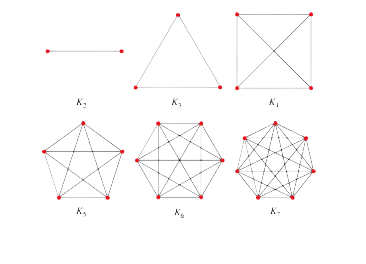
\includegraphics[scale=0.5]{k}
  \end{center}

  Una colección de grafos que es cerrada bajo isomorfismos se llama una \textbf{propiedad del grafo}.

  Una aplicación

  $$ g \ : \ \text{Conjunto de grafos }\to \mathbb{R} $$

  que asigna los mismos valores a dos grafos isomorfos se llama un \textbf{invariante del grafo.}
\end{definition}

\begin{definition}
  { \color{turquoise} \textbf{Grafos bipartitos}}

  Un grafo $G=(V,E)$ es \textbf{bipartito} si $V = V_1 \cup V_2, \ V_1 \ne \emptyset, \ V_2 \ne \emptyset, \ V_1 \cap V_2 = \emptyset$. y

  $$ \forall (v_1,v_2) \in E \implies \text{se cumple una de }\left\{ \begin{array}{l}
    v_1 \in V_1, \ v_2 \in V_2\\
    v_1 \in V_2, \ v_2 \in V_1
  \end{array} \right. $$

  Un \textbf{grafo completo bipartito} es un grafo bipartito con $E=V_1 \times V_2$, es decir, que contiene a todas las aristas posibles con un extremo en $V_1$ y otro en $V_2$. Si $|V_1| =r$ y $|V_2| =s$, al correspondiente grafo bipartito se le llama $K_{r,s}$.

  \begin{center}
    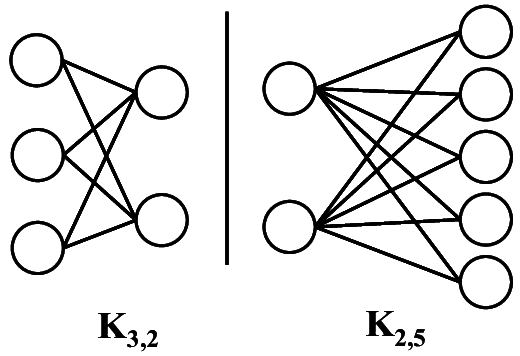
\includegraphics[scale=0.7]{k2}
  \end{center}
\end{definition}

\newpage

\begin{definition}
  { \color{turquoise} \textbf{Paseo}}

  Llamamos \textbf{paseo} (o tour) en un grafo $G=(V,E)$ a una sucesión alternante de aristas de $ E $ y vértices de $ V $, de la forma

  $$ (v_1,(v_1,v_2), v_2, (v_2, v_3), v_3, ..., v_{k-1}, (v_{k-1}, v_k), v_k) $$

  que comienza en un vértice y termina en otro, tal que cada arista incide en el nodo anterior y posterior de la sucesión.

  Se dice que el paseo \textbf{conecta} (o une) el primer y el último vértice, $v_1$ y $v_k$.

  Si $v_1 = v_k$, se dice que el paseo es \textbf{cerrado}.
\end{definition}

\begin{definition}
  { \color{turquoise} \textbf{Cadena}}

  Una \textbf{cadena (o camino)}, que a veces se le llama cadena elemental, es un grafo $P = (V,E)$ definido por $V = \{ v_1, ..., v_n \}$ y $E = \{ (v_1,v_2), (v_2,v_3), ..., (v_{n-1}, v_n) \}$, es decir, una sucesión alternante ede aristas y cértices distintos que comienza en un vértice y termina en otro, tal que cada arista incide en el nodo anterior y posterior de la sucesión.

  Se dice que $p$ conecta (o une) $v_1$ con $v_n$. Al camino con $ m $ aristas se le suele denominar $P_m$.

  Llamamos \textbf{longitud de la cadena} al número de aristas que la componen. Un subgrafo de $G$ que sea cadena (camino) se denominará cadena (camino) en el grafo $G$.
\end{definition}

\begin{definition}
  { \color{turquoise} \textbf{Ciclo}}

  Un \textbf{ciclo} (o ciclo elemental) es un grafo $C=(V,E)$ definido por $V= \{ v_1,...,v_n \}\ (n \geq 3)$ y $E= \{ (v_1,v_2), (v_2, v_3), ... , (v_{n-1}, v_n), (v_n, v_1) \}$, es decir, una cadena más una arista entre los vértices unidos por la cadena. Al ciclo con $ n $ nodos (y aristas) se le suele denominar $ C_n $.

  Llamamos \textbf{longitud del ciclo} al número de aristas que lo componen.

  Un subgrafo de $G$ que sea un ciclo se denominará ciclo en el grafo $ G $
\end{definition}

\begin{definition}
  { \color{turquoise} \textbf{Cociclo}}

  Dado un grafo $G=(V,E)$ y un conjunto $B \subseteq V$, se llama \textbf{cociclo} asociado a $ B $ al conjunto de aristas que inciden en $ B $ y en $ V \setminus B $

  $$ \omega (B) = \{ (v_1,v_2) \in E \ : \ v_1 \in B , \ v_2 \not \in V \text{ o bien }v_2 \in B, \ v_1 \not \in B \} $$

  Habitualmente se usa la notación $\omega (v)$ para referirse a $ \omega (\{ v \}) $
\end{definition}

\begin{definition}
  { \color{turquoise} \textbf{Matriz de adyacencia}}

  Dado $G = (V,E)$ con $V= \{ v_1,...,v_n \}$, la \textbf{matriz de adyacencia} $M_{n \times n}=m_{i,j}$ con

  $$ m_{ij} = \left\{ \begin{array}{l}
    1 \text{ si } v_i \text{ es extremo de } e_j\\
    0 \text{ en otro caso.}
  \end{array} \right. $$
\end{definition}

\begin{definition}
  { \color{turquoise} \textbf{Matriz de incidencia}}

  Dado un grafo $G=(V, E)$ con $V=\left\{v_{1}, \ldots, v_{n}\right\}$ y $E=\left\{e_{1}, \ldots e_{m}\right\}$, la \textbf{matriz de incidencia} (vértice-arista) es $M_{n \times m}=\left(m_{i j}\right)$ con
$$
m_{i j}= \begin{cases}1 & \text { si } v_{i} \text { es extremo de } e_{j} \\ 0 & \text { en otro caso }\end{cases}
$$
\end{definition}

También se puede representar un grafo mediante una matriz de enteros, de tamaño $m \times 2$, cuyas filas contienen los extremos inicial y final de las aristas del grafo.

\begin{proposition}
  $G=(V,E)$ es un grafo bipartito si y sólo si no contiene ciclos de longitud impar.
\end{proposition}

\begin{demonstration}
  $$ \implies \text{Suponiendo G bipartito} $$

  Sea $C$ un ciclo en $G$, tomamos $v \in G$ (sin pérdida de generalidad) $v_1 \in V_1$ y $v_2$ vecino de $v_1$. Si $v_1 \in N(v_1) \implies v_2 \in V_2$, y vamos buscando de manera iterada vecinos.

  En algún momento alcanzamos $V_k$ (el último nodo), lo cual nos obliga a que $v_k \in V_2$ y eso sólo puede ocurrir si $k=2$ (no entiendo muy bien esta dem sinceramente)

  $$ \impliedby \text{Suponiendo que no contiene ciclos de longitud par} $$

  Elegimos un nodo cualquiera $v \in V$ y lo llamamos '+'. A todos los nodos que sean vecinos de $v$, los llamamos '-', y nos olvidamos de $v$. Sucesivamente iteramos con este método, cambiando de signo.

  Al final, o bien se nos acaban los nodos o bien un nodo recibe el signo más y menos simultáneamente. Si alguno tiene longitud impar, entonces nos encontraremos con este caso. Los signos positivos serían un grupo del bipartito y los negativos los otros, al haber un elemento que exista en ambos, se tiene una contradicción.

* INCISO, ESTA IMPLICACIÓN SE HA COMPLICADO MUCHO, ESTA ES UNA IDEA PERO ESTÁ INCOMPLETA

\end{demonstration}

\begin{definition}
  { \color{turquoise} \textbf{Totalmente unimodular}}

  Una matriz es \textbf{totalmente unimodular (TU)} si todos sus menores valen $0$, $1$ o $-1$.
\end{definition}

\begin{proposition}
  Un grafo es bipartito si y sólo si sus matrices de incidencia son totalmente unimodular
\end{proposition}


\begin{demonstration}
  $$ \implies  $$

  Vamos a demostrar que no contienen ciclos impares y, por lo tanto, será bipartito. Llamemos $M$ a una matriz de incidencia genérica (el resto se obtienen permutando filas y columnas, con lo que no perdemos la generalidad).

  Supongamos que $M$ contienen un ciclo impar. La submatriz obtenida de los nodos y aristas del nodo es

  $$ \left[ \begin{array}{ccccc}
    1 & 0 &  & 0 & 1\\
    1 & 1 & \vdots  & 0 & 0\\
    0 & 1 &  & 0 & 0\\
     &  & \hdots &  & \\
    0 & 0 &  & 1 & 0\\
    0 & 0 &  & 1 & 1
  \end{array} \right] $$
\end{demonstration}


\begin{definition}
  { \color{turquoise} \textbf{Entorno}}

  Dado $G=(V, E)$, llamamos \textbf{entorno (o vecindario)} de un nodo $v$ al conjunto $N(v):=\{u \in V:$ $(u, v) \in E\}$
Decimos que un vértice $v$ \textbf{incide} en una arista $e$ si $v$ es uno de los extremos de $e$.
\end{definition}






\chapter{Conexión}


\begin{definition}
  { \color{turquoise} \textbf{Unión de grafos}}

  Se define la unión de los grafos $\left(V_{1}, E_{1}\right)$ y $\left(V_{2}, E_{2}\right)$ como el grafo $\left(V_{1} \cup V_{2}, E_{1} \cup E_{2}\right)$.
\end{definition}

\begin{definition}{ \color{turquoise} \textbf{Conexión}}


  Un grafo es \textbf{conexo} si cualquier par de vértices (distintos) están conectados por una cadena. Un grafo que no es conexo suele llamarse \textbf{disconexo} (o desconectado).

  Diremos que un grafo trivial es también conexo.

\end{definition}

Definimos en $V$ la relación siguiente:

$$
\forall v_{1}, v_{2} \in V, \quad i \complement j \Leftrightarrow\left\{\begin{array}{l}
v_{1}=v_{2} \\
\text { existe una cadena en } \mathrm{G} \text { que conecta } v_{1} \operatorname{con} v_{2}
\end{array}\right.
$$

$\complement$ es una \textbf{relación de equivalencia}, de forma que $V \mid \complement$ constituye una partición de $V$, cada una de cuyas clases de equivalencia se denomina \textbf{componente conexa}.

\begin{proposition}
  Un grafo conexo $G=(V, E)$ verifica $m \geq n-1$.

\end{proposition}

\section{Algoritmo basado en las potencias de la matriz de adyacencia}

Si se calcula $C=\sum_{k=1}^{n-1} M^{k}$, donde $M$ es la matriz de adyacencia de $G$, la entrada $c_{i j}$ será positiva si y sólo si $v_{i}$ y $v_{j}$ pertenecen a la misma componente conexa. La existencia de ceros en la matriz $C$ indicaría que $G$ no es conexo.

\section{Algoritmo basado en sumas lógicas (Tarjan)}


Se define la suma lógica $\oplus$ de bits de la forma siguiente:

\begin{center}
  \begin{tabular}{|c|ll|}
  \hline$\oplus$ & 0 & 1 \\
  \hline 0 & 0 & 1 \\
  1 & 1 & 1 \\
  \hline
  \end{tabular}

\end{center}

\begin{center}
  \textbf{Paso 1}
\end{center}

Inicialización: $\quad S:=M, i:=1, c:=1$.


\begin{center}
  \textbf{Paso 2}
\end{center}

$C(c):=\left\{v_{i}\right\}$


\begin{center}
  \textbf{Paso 3}
\end{center}

Si $s_{i j}=0 \quad \forall j>i$, ir al paso 4.

En otro caso, encontrar el primer $j>i$ tal que $s_{i j}=1$, sustituir la fila $i$ y la columna $i$ de $S$ por la suma lógica de las filas $i$ y $j$, marcar la fila $j$ y la columna $j$ de $S$ y sustituir todas sus entradas por 0, hacer $C(c):=C(c) \cup\left\{v_{j}\right\}$ y volver al Paso 3 .


\begin{center}
  \textbf{Paso 4}
\end{center}

Hacer $c:=c+1$, encontrar $k>i$ que no haya sido marcada, hacer $i:=k$ y volver al paso 2.

PARAR si tal $k$ no existe.

Las componentes conexas del grafo vienen dadas por los conjuntos $C(q), q=1, \ldots, c-1$, que se calculan en el algoritmo.


\begin{proposition}
  Los vértices de un grafo conexo pueden ser numerados de forma que los subgrafos $G_{\left\{v_{1}, \ldots, v_{i}\right\}}, i=$ $1, \ldots, n$, sean todos grafos conexos.
\end{proposition}


\begin{definition} { \color{turquoise} \textbf{Separador}}

  Dado $G=(V, E)$ conexo y un subconjunto de nodos $B \subseteq V$, si el subgrafo inducido $G_{V \backslash B}$ es disconexo, $B$ se llama un \textbf{separador} de $G$.
\end{definition}

\begin{definition}
  { \color{turquoise} \textbf{Vértice de corte y puente}}


  Si un conjunto de un solo vértice $B=\{v\}$ es separador, $v$ se llama \textbf{vértice de corte.}

  Dado $G=(V, E)$ conexo, si $(V, E \backslash\{e\})$ es disconexo, la arista $e$ se denomina \textbf{puente.}
\end{definition}

\begin{definition}
  { \color{turquoise} \textbf{k-conexidad}}

  Un grafo $G=(V, E)$ es $k$\textbf{-conexo} con $k \in\{1, \ldots, n-1\}$, si todos los subgrafos inducidos por conjuntos de nodos $B$ con $|V \backslash B|<k$ son conexos.
\end{definition}

\begin{definition}
  { \color{turquoise} \textbf{Conectividad}}


  Se llama \textbf{conectividad} de $G$ y se denota $\kappa(G)$ al mayor entero $k$ tal que $G$ es $k$-conexo. Un grafo disconexo tendrá conectividad $0.$
\end{definition}


\begin{proposition}
  Un grafo $G$ es 2-conexo si y sólo si puede construir una sucesión de grafos $G_{0}=C_{n}, G_{1}, \ldots, G_{a}=G$ en la cual $G_{i}=\left(V_{i}, E_{i}\right)$ es obtenido de $G_{i-1}=\left(V_{i-1}, E_{i-1}\right)$ mediante la unión de un camino $\left(v_{i_{1}}, \ldots, v_{i_{i}}\right)$ con $\left\{v_{i_{1}}, \ldots, v_{i_{k_{i}}}\right\} \cap V_{i-1}=\left\{v_{i_{1}}, v_{i_{k_{i}}}\right\}$.

\end{proposition}


\begin{definition} { \color{turquoise} \textbf{Arista conectividad}}

  El grafo $G=(V, E)$ es $k$\textbf{-arista-conexo} (o $k$-conexo por aristas) si todos los subgrafos $(V, E \backslash F)$ con $|F|<k$ son conexos.

  Se llama \textbf{arista-conectividad (o conectividad por aristas)} de $G$ conexo y se denota $\lambda(G)$ al mayor entero $k$ tal que $G$ es $k$-arista-conexo.

\end{definition}

\begin{proposition}
  En todo grafo (conexo) $G$ se verifica $\kappa(G) \leq \lambda(G)$.
\end{proposition}

\begin{definition}
  { \color{turquoise} \textbf{Separar}}

  Dados dos conjuntos de vértices $A$ y $B$ en $G=(V, E)$, otro conjunto de vértices $W$ \textbf{separa} $A$ de $B$ si cada camino que une un vértice de $A$ y uno de $B$ contiene un vértice de $W$.

\end{definition}

\begin{theorem}
  { \color{turquoise} \textbf{De Menguel}}


  Sea $G=(V, E)$ un grafo y $A, B \subseteq V$. Entonces el mínimo número de vértices que separan $A$ de $B$ en $G$ es igual al máximo número de caminos disjuntos que conectan $A$ y $B$.

\end{theorem}

\begin{proposition}
  Sean $u$ y $v$ dos vértices diferentes de $G .$ Si $(u, v) \notin E$, el mínimo número de vértices distintos de $u$ y $v$ que separan $u$ de $v$ en $G$ es igual al número máximo de caminos con interior disjunto que conectan $u$ y $v$ en $G$
\end{proposition}

\begin{theorem}
  { \color{turquoise} \textbf{De Menguel II}}


  Un grafo es $k$-conexo si y sólo si contiene $k$ caminos de interior disjunto entre cualquier par de vértices distintos.

\end{theorem}


\chapter{Arboles}

\begin{definition}
  { \color{turquoise} \textbf{Árboles y propiedades}}

  Diremos que un grafo $G=(V, E)$ es un \textbf{árbol} si es \textbf{conexo y no contiene ciclos.}

Un \textbf{árbol generador} de un grafo $G=(V, E)$ es un subgrafo parcial conexo y sin ciclos. Un \textbf{bosque} es un grafo $G=(V, E)$ sin ciclos.

En un árbol, los nodos con grado de incidencia 1 se denominan \textbf{hojas.}
\end{definition}

\begin{theorem}
  { \color{turquoise} \textbf{Teorema de caracterización de árboles}}
  Sea $G=(V, E)$. Son equivalentes:

  (1) $G$ es conexo y sin ciclos.

  (2) Entre cada par de vértices distintos de $V$ existe una única cadena.

  (3) $G$ es conexo y $m=n-1$.

  (4) $G$ no contiene ciclos y $m=n-1$.

  (5) $G$ está minimalmente conectado.

  (6) $G$ no contiene ciclos y si añadimos una arista entre dos vértices no adyacentes cualesquiera de $V$, el grafo que se obtiene contiene un único ciclo.
\end{theorem}

\begin{demonstration}
  $$ 1 \implies 2 $$

  Tengo que $ G $ es un grafo conexo y con ciclos. Vamos a demostrar que existe una única cadena entre $u$ y $v$.

  Como es conexo, existe una cadena entre $u$ y $v$. Para comprobar la unicidad, usaremos la ausencia de ciclos. Si existieran dos cadenas diferentes, su yuxtaposición contendría (al menos) un ciclo, con lo cual no pueden existir.

  $$ 2 \implies 3 $$

  Si se tiene que entre cada par de vértices distintos existe una única cadena, se tiene por definición que $G$ es conexo. Sólo hay que demostrar que $m=n-1$.

  Utilizaremos una proposición que dice que $G\ conexo \implies m \geq n-1$ y procederemos con inducción sobre el número de nodos.

  Para $n=1$, hay cero aristas. Para $n=2$, sólo puede haber una arista. Para $n > 2$, asumamos que se cumple para $n-1$. Eliminamos una arista (cualquiera) del grafo y dado que esa cadena es la única que conecta $u$ con $v$, ahora cada uno pertenece a componentes conexas con $n_1$ y $n_2$ nodos y $m_1$ y $m_2$ aristas respectivamente, que siguen cumpliendo la propiedad de hipótesis, luego $m_1=n_1-1$ y $m_2 = n_2-1$, con lo que en $G$, $n = m + n_2 = m_1 + 1 + m_2 + 1 = (m_1+m_2+1)+1=m+1$.

  $$ 3 \implies 4 $$

  Si existiera un ciclo en $G$, retirando una arista del ciclo no podría desconectar el grafo. Tendría un grafo conexo con $n$ nodos y $m-1$ aristas. Como $m=n-1$, me quedaría que $m-1=n-1 \implies m=n$, que es una contradicción.

  $$ 4 \implies 5 $$

  Basta demostrar que el grado es conexo, porque como se tiene que $m=n-1$ y todo grafo conexo cumple $m \geq  n-1$, no podría estar conectado.

  Supongamos que $G$ tiene $s$ componentes conexas, $(V_1,E_1), ..., (V_s, E_s) \to n_1\ nodos,\ m_i\ aristas$.

  Cada componente conexa es acíclica y conexa, luego cumple la propiedad 1 del teorema, cumpliendo también 2 y 3, y cumpliendo 3 cumple que $m_i=n_i-1\ \forall i$.

  Se tiene que $n= \sum_{i=1}^{s}n_1= \sum_{n=1}^{s}(m_i+1)=s+ \sum_{i=1}^{s}m_i = m+s $

  $$ 5 \implies 6 $$

  Añadir una arista cierra un ciclo con la cadena que conecta sus extremos. Si cerráramos dos o más ciclos, retirar una de las arista no desconectaría el grafo de partida.


  $$ 6 \implies 1 $$

  Supongamos que el grado es acíclico y la adición de una arista da un único ciclo. Por hipótesis, no se contienen ciclos, y la condición de que añadir una arista crea un ciclo implica que, entre esos dos nodos, ya había previamente una cadena, con lo que el grafo es conexo.
  \end{demonstration}
\begin{definition}
  { \color{turquoise} \textbf{Raíz y árboles con raíz}}

  En un árbol podemos distinguir un nodo cualquiera que pasará a llamarse \textbf{(nodo) raíz} $r$. El par compuesto por árbol y raíz se llamará entonces \textbf{árbol con raíz} o enraizado. El resto de nodos con grado de incidencia mayor que uno se llamarán \textbf{nudos}.
\end{definition}

\begin{definition}
  { \color{turquoise} \textbf{Predecesores y comparables}}

  Cada nodo $ v \ne r $ del árbol estará conectado a $ r $ mediante un único camino ($ r,v_1,...,v_k,v $).

  Diremos entonces que los nodos $ r,v_1,...,v_k $ son \textbf{predecesores} de $ v $ en el árbol y que $ v $ es sucesor de estos nodos. La relación de precedencia $ u \leq v \iff u $ precede a $ v $ o bien $ u = v $ induce un orden parcial\footnote{reflexivam antisimética y transitiva} en los nodos del árbol enraizado. Si $ u \leq v $ o $ v \leq u $, diremos que $ u $ y $ v $ son \textbf{comparables.}
\end{definition}

\begin{definition}
  { \color{turquoise} \textbf{Alturas}}

  Diremos que la raíz del árbol enraizado está a \textbf{nivel cero}. Los vecinos de la raíz decimos que están a \textbf{nivel uno}. Cuando suben al nivel seis, pillan ulti y te pueden oneshotear.

  Los vecinos de los de nivel uno son de nivel dos... etc. Llamaremos \textbf{altura} del árbol enraizado al máximo de los niveles de sus nodos.
\end{definition}



\begin{proposition}
  Todo árbol con $ n \geq 2 $ tiene al menos dos hojas
\end{proposition}

\begin{demonstration}
  Sea $ h $ el número de hojas del árbol $ G $, sabemos que $ m = n-1 $


  $$h + \sum_{no\ hojas} g(v)_{\geq 2} = \sum_{hojas} g(v) + \sum_{no\ hojas} g(v)  = \sum_{v \in V} {g(v)} = 2*m = 2n-2 $$
  $$ h = 2n-2 (\geq 2(n-h)) \implies h \geq 2 $$
\end{demonstration}



\begin{definition}
  { \color{turquoise} \textbf{Árbol binario}}

  Un \textbf{árbol binario} es aquél cuyo grado tienen 1 o 3 excepto un único nodo que tiene grado 2. Llamaremos \textbf{raíz del árbol binario} al nodo de grado 2.
\end{definition}


\begin{proposition}
  El número de vértices de un árbol binario es impar.
\end{proposition}
\begin{demonstration}
  $$ \sum_{v \in V}^{} g(v) = 2m = 2n-2 $$
  $$ \sum_{v \in V}^{} g(v) = h+2+3(n-h-1) $$
  $$ 2-n-2 = 2+3n-2h-3 $$
\end{demonstration}



\begin{proposition}
  La altura de un árbol binario está comprendida entre $ \lceil log_2(n+1)-1 \rceil $ y $ (n-1)/2 $
\end{proposition}

\begin{demonstration}
  Es fácil comprobarlo haciendo una representación de los posibles árboles de máxima altura y de mínima altura.

  Para hacerlo ha utilizado un trick \textbf{bastante importante,}
  $$ \sum_{i=0}^{k}2^i=2^{k+1}-1 $$
\end{demonstration}


\begin{definition}
  { \color{turquoise} \textbf{Red}}

  Una \textbf{red} es una terna $(V,E, \mathcal{L})$ formada por un grafo $(V,E)$ y una función $\mathcal{L} \ : \ E \to R$, llamada \textbf{función de peso (longitud, coste... tiene muchos nombres)}.
\end{definition}


\begin{definition}
  Dada una red $(V, E \mathcal{L})$ y un árbol generador, $T=(V, E_T)$, se define el \textbf{peso del árbol} como

  $$ \mathcal{L}(T) = \sum_{e \in E_T}\mathcal{L}(e) $$
\end{definition}

La búsqueda del árbol generador de peso mínimmo (o árbol generador minimal) en $ G $ es la resolución del problema.

\begin{proposition}
  Considérese una red $G= (V,E, \mathcal{L})$ y un árbol generador de $ G, \ T=(V, E_T) $. Las siguientes afirmaciones son equivalentes:

  \begin{itemize}
    \item $ T $ es un árbol generador minimal.
    \item Dada cualquier arista $a \in E \setminus E_T$ y cualquier otra arista $ e \in E_T $ perteneciente al único ciclo del grado $(V E_T \cup \{ a \}) $ se verifica $ \mathcal{e} \leq \mathcal{a} $
    \item Para cualquier arista $ e \in E_T, \ \mathcal{L}(e) \leq \mathcal{L}(a) \hspace{0.5cm} \forall a \in \omega (V_1^e) $, donde este último es el cociclo en el grafo $G$ asociado a una componente conexa cualquiera de $(V, E_T \setminus \{ e \})$
  \end{itemize}
\end{proposition}
\begin{demonstration}
  $$ 1 \implies 2 $$


  $$ 2 \implies 3 $$
\end{demonstration}




\section{Algoritmo de Kruskal}

\begin{center}
  \textbf{Paso 1}
\end{center}

    Ordenar las aristas de $ E $ en orden ascendente de su peso:
    $$ V = \{v_1,...,v_n\},\ T^* = (V, \emptyset) \hspace{1cm} E := \{e_1,...,e_m\}:\ \mathcal{L}(e_i) \leq \mathcal{L}(e_i+1) \forall i < m $$

    \begin{center}
      \textbf{Paso 2}
    \end{center}

    Añadir $ n-1 $ aristas a $ T^* $ sucesivamente (en el orden de sus pesos) sin que se formen ciclos.

    \section{Algoritmo de Prim}

\begin{center}
  \textbf{Paso 1}

\end{center}

    Elegir un vértice $ r \in V $ y hacer $ V_1 = \{r\},\ V_2 = V \setminus \{r\} $.

\begin{center}
  \textbf{Paso 2}
\end{center}

    Añadir al árbol la arista de menor peso de $ w(V_1) $, digamos $ (v_1,v_2) $ con $ v_1 \in V_1 $ y $ v_2 \in V_2 $. Añadir $ v_2  $ a $ V_1 $ y borrar $ v_2  $ de $ V_2 $.

\begin{center}
  \textbf{Paso 3}

\end{center}

    Si $ |V_1| = n $ parar. Si no, volver al Paso 2.

\chapter{Caminos más cortos, recorridos por arsitas y vértices}


\begin{definition}
  { \color{turquoise} \textbf{Longitud de un camino}}

  Sea $(V, E, \ell)$ una red con $G=(V, E)$ y $P$ un camino en $G$. Se define la \textbf{longitud del camino} $P$ como

  $$
  \ell(P):=\sum_{a \in P} \ell(a)
  $$

\end{definition}

El problema del camino más corto (CMC) entre $v_{i}$ y $v_{j}$ en $G$ es

$$
\begin{aligned}
\min\ & \ell(P) \\
\text { s.a } & P \text { es un camino que une } v_{i} \text { con } v_{j}
\end{aligned}
$$

En lo que sigue, para una arista $e=\left(v_{i}, v_{j}\right)$ notaremos indistintamente $\ell\left(v_{i}, v_{j}\right), \ell_{e}, \ell_{i j} .$ También supondremos que la red es conexa y que $\ell_{e} \geq 0\ \forall e \in E$.

\begin{proposition}
  Dado un camino más corto de $v_{a}$ a $v_{b}$, todo subcamino de éste que conecte $v_{i}$ con $v_{j}$ es un camino más corto entre $v_{i}$ y $v_{j}$

\end{proposition}

\begin{demonstration}
    Si hubiera un camino más corto $ P_1 $ entre $ v_i $ y $ v_j $ que el subcamino $ P_2 $ entre $ v_i,v_j $, reemplazando $ P_2 $ por $ P_1 $ obtenemos o bien 1. o 2.:
    \begin{enumerate}
        \item Un camino más corto que el camino más corto con lo que tenemos una contradicción.
        \item Un paseo que contiene ciclos, la eliminación de estos ciclos nos deja un camino más corto que el camino más corto, de nuevo una contradicción.
    \end{enumerate}
\end{demonstration}



\begin{theorem}
  El vector $d=\left(d_{1}, d_{2}, \ldots, d_{n}\right)$ que contiene longitudes de caminos que conectan el nodo $v_{s}$ con todos los nodos $v_{1}, v_{2}, \ldots, v_{n}$ de una red, con $d_{s}=0$, mide las longitudes de los caminos más cortos entre $v_{s}$ y todos los demás nodos si y sólo si

  $$
  d_{j}-d_{i} \leq \ell_{i j} \forall\left(v_{i}, v_{j}\right) \in E
  $$
\end{theorem}

\begin{demonstration}
    $ \impliedby $

    Supongamos $ d_j > d_i + l_{ij} $, entonces, podemos crear un camino más corto a $ j $ yuxtaponiendo el camino a $ i $ y la arista que une $ i $ con $ j $ si no se forman ciclos, si se formaran, basta con quitarlo y aún así tendríamos un camino más corto a $ j $. En ambos casos tenemos una contradicción.

    $ \implies $

    Sea $ j \in V $ cualquiera, sea $ P $ un camino cualquiera de $ s $ a $ j $, ¿se cumple que $ l(p) \geq d_j $? Si $ P = (s = i_0,i_1,...,i_{q}=j) $ tenemos que:

    $$ d_{i_1}-d_{i_0} \leq l_{i_0i_1} \hspace{5mm} d_{i_2}-d_{i_1} \leq l_{i_1i_2} \hspace{5mm} ...$$

    Sumando todo obtenemos que $d_j-\underbrace{d_{s}}_{0} = d_{i_q}-d_{i_0} \leq \sum\limits_{k}^{}l_{i_{k}i_{k+1}} = l(P)$

\end{demonstration}



\begin{theorem}
  Supongamos que el vector $d=\left(d_{1}, d_{2}, \ldots, d_{n}\right)$ contiene longitudes de caminos que conectan el nodo $v_{s}$ con todos los nodos $v_{1}, v_{2}, \ldots, v_{n}$ de una red, con $d_{s}=0$. Sea $V^{\prime}$ un conjunto de vértices para el cual

  (a) $v_{s} \notin V^{\prime}$

  (b) si $v_{i} \notin V^{\prime}, d_{i}$ es la longitud de un camino más corto de $v_{s}$ a $v_{i}$,

  (c) si $v_{i} \in V^{\prime}, d_{i}=\min \left\{d_{j}+\ell_{j i}: \quad v_{j} \notin V^{\prime}, v_{j} \in N\left(v_{i}\right)\right\}$ Sea $v_{j} \in V^{\prime}$ tal que

  $$
  d_{j}=\min \left\{d_{i}: \quad v_{i} \in V^{\prime}\right\}
  $$

  Entonces $d_{j}$ es la longitud de un camino más corto de $v_{s}$ a $v_{j}$.
\end{theorem}

\begin{demonstration}
    Sea $ P $ camino entre $ s $ y $ j  $, ¿ $ l(p)\geq d_j $ ? De este camino $ (v_{s},v_{a},v_{b},...,v_{j}) $ sabemos que:
    \begin{itemize}
        \item $ v_{s} \not \in V' $
        \item $ v_j \in V' $
    \end{itemize}
    Si $ P_{2} $ es el subcamino desde $ s $ hasta el primer nodo de $ V' $ con último coste $ (v_{i_1},v_{i_2}) \in w(V') $, entonces:
    $$ l(P) \geq l(P_2) =\underbrace{l(P_1)}_{\text{longitud del sucamino que une $ s $ y $ v_{ij} $}}+l_{i_1i_2} \geq d_{i_1} + l_{i_1}l_{i_2} \geq _{(c)} d_{i_2} \geq d_j$$
\end{demonstration}


\section{Algoritmo de Dijkstra}

\begin{center}
\textbf{Paso 1}
\end{center}


$d_{s}:=0 \quad d_{i}:=\ell_{s i} \forall v_{i} \in N\left(v_{s}\right) \quad d_{i}:=\infty$ en otro caso. $p(i):=s \quad \forall v_{i} \in N\left(v_{s}\right), \quad p(i):=0$ en otro caso, $\quad V^{\prime}:=V \backslash\left\{v_{s}\right\}$


\begin{center}
\textbf{Paso 2}
\end{center}

Buscar un nodo $v_{j} \in V^{\prime}$ tal que $d_{j}=\min \left\{d_{i}: v_{i} \in V^{\prime}\right\} .$ Hacer $V^{\prime}:=V^{\prime} \backslash\left\{v_{j}\right\}$.

\begin{center}
\textbf{Paso 3}
\end{center}

Para todo $v_{i} \in N\left(v_{j}\right) \cap V^{\prime}:$ si $d_{j}+\ell_{j i}<d_{i}$ entonces:

$$
d_{i}:=d_{j}+\ell_{j i}, \quad p(i):=j
$$

Si $V^{\prime} \neq \emptyset$, volver al Paso 2 .



\begin{definition}
  { \color{turquoise} \textbf{Tour eureliano y grafo euleriano}}

  Dado un grafo $G=(V, E)$, se llama \textbf{tour euleriano (o recorrido euleriano)} a un paseo cerrado que atraviesa cada arista de $E$ exactamente una vez. Un grafo que admite un recorrido euleriano se denomina \textbf{grafo euleriano.}
\end{definition}

\begin{theorem}
  Un grafo conexo es euleriano si y sólo si todos los vértices son pares.
\end{theorem}

\section{Algoritmo de Fleury}

\begin{center}
\textbf{Paso 1}
\end{center}

Comenzando con una copia del grafo, $G^{\prime}=\left(V^{\prime}, E^{\prime}\right)$, elegir cualquier vértice $i \in V^{\prime}$.

\begin{center}
\textbf{Paso 2}
\end{center}

Si existe una arista $(i, j) \in E^{\prime}$ que no sea puente en $G^{\prime}$, elegirla. En otro caso, elegir cualquier arista $(i, j)$ de $E^{\prime}$

\begin{center}
\textbf{Paso 3}
\end{center}

Anotar la arista $(i, j)$ en el paseo y eliminarla de $E^{\prime} .$ Si $E^{\prime}=\emptyset$, FIN. En otro caso, hacer $i:=j$ y volver al paso 2 .

\section{Algoritmo de Hierholzer}

\begin{center}
\textbf{Paso 1}
\end{center}

Comenzando con una copia del grafo, $G^{\prime}=\left(V^{\prime}, E^{\prime}\right)$, elegir cualquier vértice $i \in V^{\prime}$.

\begin{center}
\textbf{Paso 2}
\end{center}

Si se puede elegir una arista $(i, j)$ de $E^{\prime}$, anotar la arista $(i, j)$ en el paseo y eliminarla de $E^{\prime} .$ Si $E^{\prime}=\emptyset$, FIN. Si $E^{\prime} \neq \emptyset$ hacer $i:=j$ y volver al paso 5

Si no se puede elegir ninguna arista $(i, j)$ de $E^{\prime}$, reemplazar $i$ por un vértice ya perteneciente al paseo en el que incida una arista de $E^{\prime} .$ Sea $(j, i), i,(i, k)$ un tramo de este paseo. Hacer $e=(j, i)$. Volver al paso 5 pero anotando la arista en el interior del paseo a continuación de $e$ y reeplazando $e$ por la arista anotada.


\begin{definition}{ \color{turquoise} \textbf{Cartero chino}}



  Dada una red $(V, E, \ell)$, a la determinación del \textbf{paseo cerrado de mínima longitud que incluye a todas las aristas} de $E$ (por lo menos una vez) se le llama \textbf{problema del cartero chino} sobre esa red.
\end{definition}

\section{Algoritmo de Dantzig}

\begin{center}
\textbf{Paso 1}
\end{center}

Hacer $k:=1$ y obtener para cada $v_{i}, v_{j} \in V$ :

$$
D(i, j):=\left\{\begin{array}{ll}
0 & \text { si } i=j, \\
\infty & \text { en otro caso, }
\end{array} \quad P(i, j):=i\right.
$$

\begin{center}
\textbf{Paso 2}
\end{center}

Para $i=1,2, \ldots, k$

$$
\begin{gathered}
D(i, k+1):=\min _{j=1, \ldots, k}\left\{D(i, j)+\ell_{j, k+1}\right\} \\
P(i, k+1):=\arg \min _{j=1, \ldots, k}\left\{D(i, j)+\ell_{j, k+1}\right\}
\end{gathered}
$$

Si $\arg \min _{j=1, \ldots, k}\left\{\ell_{j, k+1}+D(i, j)\right\} \neq i$,

$$
P(k+1, i):=P\left(\arg \min _{j=1, \ldots, k}\left\{\ell_{j, k+1}+D(i, j)\right\}, i\right)
$$

Si $\arg \min _{j=1, \ldots, k}\left\{\ell_{j, k+1}+D(i, j)\right\}=i$,

$$
\begin{gathered}
P(k+1, i):=k+1, \\
D(k+1, i):=D(i, k+1)
\end{gathered}
$$

\begin{center}
\textbf{Paso 3}
\end{center}

Para cada $i, j=1, \ldots, k$ hacer

$$
D(i, j):=\min \{\underbrace{D(i, j)}_{A}, \underbrace{D(i, k+1)+D(k+1, j)}_{B}\} ;
$$

Si el mínimo es B, hacer $P(i, j):=P(k+1, j)$. Hacer $k:=k+1 .$ Si $k<n$, volver al Paso 2

El problema del cartero chino se resuelve mediante el siguiente procedimiento:

  1. Usar el algoritmo de Dantzig para calcular las longitudes de los caminos más cortos entre cada par de nodos de la red.

  2. Calcular el coste de todos los emparejamientos posibles sumando las longitudes obtenidas en el paso anterior.

  3. Seleccionar el emparejamiento de menor coste.

  4. Duplicar, en la red original, todas las aristas pertenecientes a los caminos más cortos para el emparejamiento elegido.

  5. En el (multi)grafo euleariano así obtenido, encontrar un ciclo euleariano usando el algoritmo de Fleury.

\begin{definition}
  { \color{turquoise} \textbf{Hamiltoniano}}
  Un ciclo en un grafo $G$ es \textbf{hamiltoniano} si \textbf{contiene a todos los vértices del grafo.} Si tal ciclo existe, diremos que el grafo es hamiltoniano.

  En un grafo $G$ un \textbf{camino hamiltoniano} es aquél que contiene a todos los vértices del grafo.

\end{definition}

Dado un grafo $G$ se obtiene el grafo clausura de $G$, denotado por $[G]$, mediante el proceso iterativo siguiente:

- Se define $G_{0}=\left(V, E_{0}\right):=G, j=0$.

- Mientras exista un par de nodos $u, v$ en $G_{j}$ tales que $(u, v) \notin E_{j}$ y $g_{G_{j}}(u)+g_{G_{j}}(v) \geq n$,

- hacer $j:=j+1$

- hacer $E_{j}:=E_{j-1} \cup\{(u, v)\}$,

- hacer $G_{j}:=\left(V, E_{j}\right)$.

\begin{theorem}
  Un grafo $G$ es hamiltoniano si y sólo si su grafo clausura $[G]$ es hamiltoniano.
\end{theorem}


\begin{demonstration}

    $ \implies $

    Directo.

    $ \impliedby $

    Reducción al absurdo: supongamos que existe un grafo no hamiltonianos cuya clausura sí es hamiltoniana.

    Sea $ G_0,...,G_k = [G] $ con $ j $ el primer índice tal que $ G_{j} $ no es hamiltoniano pero $ G_{j+1} $ sí lo es. La última arista añadida, digamos que es $ (v_1,v_n) \not \in E_j $ y $ (v_1,v_n) \in E_{j+1} $, tiene que estar en el ciclo hamiltoniano de $ G_{j+1} $. Sea este ciclo $ v_1,...,v_n,v_1 $.

    Retirando $ (v_1,v_n) $ de nuevo, se sigue que en $ G_j $ existía un camino hamiltoniano $ (v_1,v_2,...,v_n) $.

    Sean $ Y = \{i \in \{3,...,n-1\} : (v_1,v_i) \in E_j\} $ (algunos de los vecinos de $ v_1 $) y $ X = \{i \in \{3,...,n-1\}:(v_n,v_{i-1}) \in E_j\} $ (los nodos a la derecha de algunos de los vectores de $ v_n $). Entonces $ |Y| = g_{G_j}(v_1) -1$ y $ |X| = g_{Gj}(v_n)-1 $ y $ |X| + |Y| \geq_{\text{por la contrucción de $ G_{j+1} $}} n-2  $.

    Como $ X,Y \subset \{3,4,...,n-1\}_{\text{con cardinal $ n-3 $}} $ y sus cardinales suman $ n-2 \implies X \cap Y \ne \emptyset \implies \exists v_{k} \in X \cap Y \implies $
    $$ \implies \left\{
    \begin{array}{l}
        (v_{k},v_1) \in E_j\\
        (v_{k-1},v_n) \in E_j
    \end{array}
    \right. $$
    Y tenemos que $ (v_1,..,v_{k-1},v_{n},v_{n-1},...,v_{k},v_{1}) $ es un ciclo hamiltoniano.
\end{demonstration}


\begin{definition}{ \color{turquoise} \textbf{Sucesión hamiltoniana}}

  Una $n$-tupla de naturales $\left(a_{1}, \ldots, a_{n}\right)$ se dice que es una \textbf{sucesión hamiltoniana} si todos lo grafos de $n$ nodos de grados $g_{1} \leq \ldots \leq g_{n}$ que cumplen $g_{1} \geq a_{1}, \ldots, g_{n} \geq a_{n}$ son hamiltonianos.
\end{definition}

\begin{theorem}{ \color{turquoise} \textbf{de Chvátal}}

  Para cualquier $n \geq 3$, una $n$-tupla de naturales $\left(a_{1}, \ldots, a_{n}\right)$ con $a_{1} \leq \ldots \leq a_{n}<n$ es una sucesión hamiltoniana si y sólo si para cada $i<n / 2$ se satisface

  $$
  a_{i} \leq i \Rightarrow a_{n-i} \geq n-i .
  $$

\end{theorem}


\begin{demonstration}

    $ \implies $

    Utilizaremos el contrarrecíproco, si tenemos un $ i < \dfrac{n}{2} $ tal que $ a_i \leq 1 $ y $ a_{n-1} < n-1 $

    %dibujo 4/11

    $ \impliedby $

    Supongamos que no es hamiltoniano. Sea $ G(V,E) $ un grafo con el mayor número posible de aristas que no es hamiltoniano con grafos $ g_{1}\leq...\leq g_n $. Esta grafo satisface la condición

    % $$ g_i \leq i \implies a_i\leq i \implies a_{n-i} \leq n-1 \implies g_{n-i} \geq n-i \forall i < n/2 $$
    % Sean $ u,v \in V $m con $ (u,v) \not \in E $ y $ g(u)+g(v) $ lo mayor posible.

    $$ g_i \leq i \implies a_i \leq g_i \leq 1 \implies a_{n-i} \geq n-1 \implies g_{n-i} \geq a_{n-i} \geq n-i $$

    De todos los $ G $ en estas condiciones elegimos uno con número máximo de aristas. Sean $ u,v \in V $ con $ (u,v) \not \in E $ con máxima suma de $ g(u)+g(v) $. Sea $ u $ el de menor grado: $ g(u) \leq g(v) $. Como $ G $ es maximal, al añadir la arista $ (u,v) $ pasa a ser hamiltoniano, luego $ \exists $ camino hamiltoniano $ u \sim v $ en $ G $:
    $$ u = v_1-v_2-...-v_n = v $$

    Como vimos ayer si $ u $ es vecino de $ v_{i} $, no puede darse que $ v $ sea vecino de $ v_{j} $, $ j<i $.

    Consideremos el conjunto de vecinos de $ u $ ($ N(u) \subset \{v_1,...,v_{n-1}\} $) y el conjunto de nodos de $ v_i $ que preceden inmediatamente en el camino a un vecino de $ u\subset \{v_1,..,v_{n-1}\} $. La existencia de un nodo en la intersección de estos 2 conjuntos implica la existencia de un ciclo ham. en $ G $, luego son disjuntos.

    La unión de estos dos conjuntos está incluida en $ \{v_1,...,v_{n-1}\} $. Uno de los conjuntos tiene cardinal $ g(u) $ y el otro $ g(v) $, como la unión es disjunta el cardinal es $ g(u) + g(v) $. Por tanto, tenemos que $ g(u)+g(v) < n \implies g(u) < \dfrac{n}{2} $

    Sea $ x \in V $ un nodo que precede en el camino a un vecino de $ u $ (y que por tanto no es vecino de $ v $). Como tomamos $ u,v $ que no fueran vecinos con máximo $ g(u)+g(v) $, tenemos que $ g(x) \leq g(u) $. En las condiciones de $ x $ tengo tantos nodos como $ |N(u)| = g(u) $. Sea $ i = g(u) $, entonces $ i<\dfrac{n}{2}, g(i) \leq i \implies g_{n-i} \geq n-i $

    Luego al menos hay  $ i+1 $ nodos  con grado  $ \geq n-i $. Como $ i = g(u) $ no todos estos nodos pueden ser vecinos de $ n $. Sea $ w \not \in N(u) $ con hgrado $ \geq n-i $.
    $$ g(w) \geq n-g(u)\ \implies \text{Contradicción con la elección de $ v $} $$

    %definicion de problema del viajante de comercio

\end{demonstration}



\begin{definition}{ \color{turquoise} \textbf{Problema del viajante}}

  Dada una red $(V, E, \ell)$, a la \textbf{determinación del ciclo hamiltoniano de mínima longitud} se le llama \textbf{problema del viajante de comercio} sobre esa red.
\end{definition}

\chapter{Grafos planos. Coloración de grafos.}

\begin{definition}{ \color{turquoise} \textbf{Coloración}}

  Una \textbf{coloración propia} (o simplemente coloración) de un grafo es una aplicación

  $$
  c: V \longrightarrow\{1,2, \ldots, \ell\}
  $$

  que hace corresponder valores diferentes a vértices adyacentes:

  $$
  \forall(u, v) \in E \rightarrow c(u) \neq c(v)
  $$

  El valor $c\left(v_{i}\right)$ es el \textbf{color} correspondiente al nodo $v_{i}$.

\end{definition}

\begin{definition}{ \color{turquoise} \textbf{Número cromático}}

  Llamaremos \textbf{número cromático} del grafo $G, \chi(G)$, al \textbf{mínimo valor} de $\ell$ que \textbf{permite una coloración} de $G$, es decir, al mínimo número de colores necesarios para colorear los vértices de forma que los extremos de cada arista tengan colores distintos.

\end{definition}

\begin{definition}{ \color{turquoise} \textbf{Crítico}}


  Se dice que un grafo $G$ es \textbf{crítico} si para cualquier subgrafo propio $H$ se verifica $\chi(H)<\chi(G)$.
\end{definition}
\newpage
\begin{proposition}{ \color{turquoise} \textbf{Metralleta de resultados}}
 Los siguientes tres resultados se cumplen:


  1. Cada grafo $G$ con $n \geq 2$ contiene un subgrafo crítico $H$ tal que $\chi(G)=\chi(H)$.

  2. Si $G=(V, E)$ es crítico, $G$ es conexo.

  3. Si $G=(V, E)$ es crítico, $\forall v \in V, g(v) \geq \chi(G)-1$

\end{proposition}

\begin{demonstration}
  \begin{center}
  \textbf{1.}
  \end{center}

  Si $G$ es crítico, hemos terminado. Si $G$ no es crítico, contiene un subgrafo (propio) $G_2$ con el mismo número cromático. Si $G_2$ es crítico, hemos terminado, si no, iteramos el proceso.

  Finalmente agotaremos la sucesión hasta un nodo o encontraremos uno crítico.

  \begin{center}
  \textbf{2}
  \end{center}

  En un grafo no conexo, el número cromático es el máximo de sus componentes conexas. El subgrafo inducido de una de las cc.cc. que de ese máximo tiene por tanto el número cromático de $gG$.

  \begin{center}
  \textbf{3.}
  \end{center}

  Si existe $v \in B$ con un número cromático $g(v) \leq \chi(G)-2$, retirando $v$ de $G$, dado que $G$ es crítico, $\chi(G_{V\setminus \{v\}}) \leq 1$.. Por tanto, existe una coloración $c$ propia de $G_{V\setminus \{v\}}$.
\end{demonstration}

\section{Algoritmo austero para colorear (no es óptimo)}

\begin{center}
\textbf{Paso 0}
\end{center}

Inicialización. Ordenar los elementos de $V: v_{1}, \ldots, v_{n}$.

\begin{center}
\textbf{Paso 1}
\end{center}

Asignar $c\left(v_{1}\right):=1$.

\begin{center}
\textbf{Paso 2}
\end{center}

Si $\left(v_{1}, v_{2}\right) \notin E$, asignar $c\left(v_{2}\right):=1$; en otro caso, asignar $c\left(v_{2}\right):=2$.

\begin{center}
\textbf{Paso 3}
\end{center}

- Si habíamos coloreado $c\left(v_{1}\right)=c\left(v_{2}\right)=1$ :

$\mathrm{Si}\left(v_{1}, v_{3}\right) \notin E \mathrm{y}\left(v_{2}, v_{3}\right) \notin E$, asignar $c\left(v_{3}\right):=1$

En otro caso, asignar $c\left(v_{3}\right):=2$ - Si habíamos coloreado $c\left(v_{1}\right)=1$ y $c\left(v_{2}\right)=2$ :

$\operatorname{Si}\left(v_{1}, v_{3}\right) \notin E$, asignar $c\left(v_{3}\right):=1$

En otro caso:

$\operatorname{Si}\left(v_{2}, v_{3}\right) \notin E$, asignar $c\left(v_{3}\right):=2$

En otro caso, asignar $c\left(v_{3}\right):=3$.

Y así sucesivamente.

\begin{proposition}
  { \color{turquoise} \textbf{Dos resultaditos}}

  El algoritmo de coloreado utiliza a lo sumo $1+\max _{v \in V}\{g(v)\}$ colores.

  En todo grafo $G$ se verifica $\chi(G) \leq 1+\max _{v \in V}\{g(v)\}$.

\end{proposition}

Dado un grafo $G$, consideremos la función

$$
P_{G}: \mathbb{N}^{*} \longrightarrow \mathbb{N}^{*}
$$

que asigna a cada valor $k$ el número de distintas coloraciones del grafo $G$ que no usen más de $k$ colores.

Está claro que $P_{G}(0)=P_{G}(1)=\ldots=P_{G}(\chi(G)-1)=0$, mientras que $P_{G}(\chi(G)), P_{G}(\chi(G)+$ 1) $\ldots \geq 1$. También está claro que $P_{G}(k) \leq P_{G}(k+1) \forall k$.

\begin{definition}
  { \color{turquoise} \textbf{Polinomio cromático}}

  Se llama polinomio cromático del grafo $G$ al polinomio de grado $n$ resultante de interpolar $\left(k, P_{G}(k)\right)$ para $k=0, \ldots, n$
\end{definition}

\begin{definition}
  { \color{turquoise} \textbf{Identificar}}

  Dado un grafo $G=(V, E)$ con $V=\left\{v_{1}, \ldots, v_{n}\right\}$ y un par de nodos $v_{i} \neq v_{j} \in V$, se llama \textbf{identificar} $v_{i}$ y $v_{j}$ a construir un nuevo grafo $G=\left(V^{\prime}, E^{\prime}\right)$ con $V^{\prime}=V \backslash\left\{v_{i}, v_{j}\right\} \cup\left\{v_{n+1}\right\}$ y $E^{\prime}=E \backslash\left(\left\{\left(v_{i}, v_{j}\right)\right\} \cup \omega\left(\left\{v_{i}, v_{j}\right\}\right)\right) \cup E^{\prime \prime}$, donde $E^{\prime \prime}=\left\{\left(v_{k}, v_{n+1}\right):\left(v_{k}, v_{i}\right) \in E \circ\left(v_{k}, v_{j}\right) \in E\right.$ ambas).
\end{definition}

\begin{theorem}
  Dado un grafo $G=(V, E)$ y un arista $(u, v) \in E$, se satisface $P_{G}(k)=P_{G_{1}}(k)-P_{G_{2}}(k)$ donde $G_{1}=(V, E \backslash\{(u, v)\})$ y $G_{2}$ es el grafo obtenido de $G$ identificando los dos vértices $u$ y $v$.
\end{theorem}

\begin{definition}
  { \color{turquoise} \textbf{Grafo plano}}

  Un \textbf{grafo plano} es $(V, E)$, un par de conjuntos finitos llamados vértices y aristas que satisfacen

  1. $V \subseteq \mathbb{R}^{2}$

  2. Cada arista de $E$ es un arco entre dos vértices distintos.

  3. Aristas diferentes tienen extremos diferentes.

  4. El interior de una arista no contiene ni vértices ni puntos de otra arista.

  Para cada grafo plano $G$, el conjunto $\mathbb{R}^{2} \backslash(V \cup E)$ es abierto. Sus regiones se llaman \textbf{caras}. Como $G$ es acotado, una de sus caras será no acotada y se denomina \textbf{cara externa}, a diferencia de las caras internas.
\end{definition}

\begin{definition}
  { \color{turquoise} \textbf{Planar}}

  Un grafo isomorfo a un grafo plano se denomina \textbf{planar}.

  Cada representación de un grafo planar como grafo plano se llama un \textbf{embutido.}
\end{definition}

Admitiremos las siguientes propiedades de cualquier embutido de $G$ :

- Dos caras diferentes son disjuntas, y sus contornos tienen intersección sólo en las aristas.

- Hay una única cara exterior.

- El interior de cada ciclo de $G$ contiene al menos una cara interna.

- Un puente pertenece al contorno de una sola cara.

- Una arista que no es puente pertenece exactamente al contorno de dos caras.

\begin{proposition}
  Un embutido de un grafo planar $G$ no tiene caras internas si y sólo si $G$ es un bosque.
\end{proposition}

\begin{theorem}
  Sea $G$ un grafo planar conexo. Consideremos un embutido de $G$ con $c$ caras. Entonces

  $$
  n-m+c=2
  $$

\end{theorem}

\begin{proposition}
  Si $G$ es un grafo planar con $n \geq 3$, entonces $m \leq 3 n-6$.

  Si además ningún subgrafo inducido de $G$ es $K_{3}$, entonces $m \leq 2 n-4$.
\end{proposition}

\begin{demonstration}
  Si $ m=1,2 $ es obvio. Si $m \geq 3$, entonces hay $2m$ 'lados disponibles'. Hay un mínimo de tres aristas en el contorno de una cara, por lo que tienes $3c \leq 2m\ \text{(disponibles)}$ caras.

  Aplicamos la fórmula de Euler:
  $$ n-m+c=2 \hspace{1cm}\to \hspace{1cm}3c=(m-n+2)3 \leq 2m $$
  $$ m \leq 3n-6 $$


  \begin{minipage}[l]{0.1\textwidth}
    
\includegraphics[scale=0.15]{wanda}
  \end{minipage}
  \begin{minipage}[l]{0.8\textwidth}
    La demostración es un poco terrible pero las culpas al teacher que nosotros nos hemos dedicado a copiar.
  \end{minipage}
\end{demonstration}

\begin{proposition}
  $K_{5}$ y $K_{3.3}$ no son grafos planares.
\end{proposition}

\begin{proposition}
  Si $G$ es planar, el grado medio de sus nodos es menor que 6 .
\end{proposition}

\begin{demonstration}
    $$ \overline{g} = \dfrac{\sum\limits_{v}^{}g(v)}{n} = \dfrac{2m}{n} \leq \dfrac{2(3n-6)}{n} = 6-\dfrac{12}{n} $$
\end{demonstration}

\begin{definition}
  { \color{turquoise} \textbf{Maximal}}


  Un grafo planar es maximal si la adición de cualquier arista lo convierte en no planar.

\end{definition}


\begin{proposition}
  Sea $F$ una cara de un embutido del grafo $G$ con al menos cuatro aristas en su contorno. Entonces hav dos vértices no advacentes entre los extremos del contorno de $F$.

\end{proposition}

\begin{demonstration}

  \begin{center}
    \custincfig{0.5\textwidth}{grafos1}
  \end{center}

  Si $A$ y $B$ fueran adyancentes su arista en el embutido estaría contenida en el exterior de la cara. Igual pasa con $C$ y $D$.

  En tal caso, añadiendo un vértice en el interior de la cara, añadiendo aristas entre este vértice y  los del contorno, con lo que tendríamos un embutido de $K_5$, lo que es una contradicción.
\end{demonstration}

\begin{proposition}
  Si $G$ es un grafo planar maximal con $n \geq 3$, el contorno de cada cara del embutido plano de $G$ tiene exactamente tres aristas.

\end{proposition}

\begin{demonstration}
  DPD. \footnote{Daniel Pedro Duque fue un importante matemático riojano que tuvo que viajar a la Unión Soviética, ya que fue destinado a un campo de concentración. Ahí, desarrolló importantes avances en teoría de grafos y optimización discreta, optimizando la cantidad óptima de judíos que ejecutar a cada día.

  En realidad, DPD significa 'demostrado por dibujito'}
\end{demonstration}

\begin{proposition}
  En todo grafo planar maximal con $n \geq 3$ se verifica $m=3 n-6$.

\end{proposition}

\begin{demonstration}
  Basta aplicar una demostración hecho previamente pero en este caso tomamos $3c = 2m$ por la proposición anterior.
\end{demonstration}

\begin{definition}
  { \color{turquoise} \textbf{Subdividir}}

  Dado un grafo $G=(V, E)$ y una arista $(u, v) \in E$, se llama \textbf{subdividir} la arista $(u, v)$ a añadir un nuevo nodo $v_{n+1}$ al grafo y reemplazar $(u, v)$ por $\left(u, v_{n+1}\right)$ y $\left(v, v_{n+1}\right)$.

\end{definition}


\begin{definition}{ \color{turquoise} \textbf{Subdivisión}}

  Se llama \textbf{subdivisión del grafo} $G$ al grafo obtenido de $G$ subdividiendo sucesivas aristas.
\end{definition}

\begin{theorem}
  { \color{turquoise} \textbf{Teorema de Kuratowski}} {\color{red} \tiny \textbf{TEOREMA IMPORTANTE DE LA REHOSTIA}}

  Un grafo es planar si y sólo si no contiene como subgrafo ninguna subdivisión de $K_{5}$ ni $K_{3,3}$.

\end{theorem}

\begin{theorem}
  Si $G$ es un grafo planar, entonces $\chi(G) \leq 4$.

  (aunque demostraremos el teorema del mapa de los cinco colores)

\end{theorem}

\begin{demonstration}
  \begin{flushright}
    (con cinco colores porque no tenemos la picha tan gorda)
  \end{flushright}

  Supongamos que existen grafos planares con $\chi(G) \geq 6$. Tomamos el menor grafo que requiera 6 o más colores. De ellos, elegimos un grafo planar $G$ con $\chi(G)=6$ cuyos subgrafos tienen todos número cromático 5 o menos (crítico).

  Utilizando un resultado anterior, planar implica que $\overline{g} < 6 \implies \exists v \in V \ : \ g(v) \leq 5$. Si $g(v) \leq 4$, G no es crítico.

  Luego elegimos $v$ son $ g(v) = 5 $. Cualquier coloración del grafo $ G $ tiene que cumplir que $ c(u_1) \ne c(u_2) \forall u_1 \ne u_2\ u_1,u_2 \in N(v)  $. En otro caso $ G $ no sería crítico.

  Ordenamos los vecinos de $v$ por el ángulo de la arista $(v, u_i)$. El nodo $ u_i $ recibe en la coloración el color i-ésimo.

  Nos fijamos en el subgrafo inducido por los nodos coloreados con los colores 1 y 3. Este grafo conecta $u_1$ y $u_3$ ya que si no fuera así podríamos alternar los colores de una de las componentes conexas. Entonces dos vecinos de $ v $ tendrían el mismo color, lo cual ya hemos visto que no puede ser.

  Podemos formar un ciclo entonces  que pasa por $v,u_1,u_3$ que contiene al menos una cara que a su vez contiene a $ u_2 $ o a $u_4$ y al otro no. Con lo queseparamos en el embutido a $ u_2 $ de $ u_4 $.

  Por el mismo razonamiento, existe un camino entre $ u_2$ y $ u_4 $. Pero ese camino tendría intersección con el que acabamos de crear, luego el grafo no sería planar y hemos llegado a una contradicción.

\end{demonstration}

\chapter{Modelo de Programación Entera (Optimización Discreta)}


Un problema de programación lineal es aquél que se puede establecer mediante la formulación

$$
\begin{cases}\min _{x} & c \cdot x \\ \text { s.a } & A x \leq b \\ & x \in \mathbb{R}_{+}^{n}\end{cases}
$$

con $c \in \mathbb{R}^{n}, A_{m \times n}=\left(a_{i j}\right), a_{i j} \in \mathbb{R} \forall i, j, b \in \mathbb{R}^{m}$.

Es decir,

$$
\begin{cases}\min & c_{1} x_{1}+c_{2} x_{2}+\ldots+c_{n} x_{n} \\ \text { s.a } & a_{11} x_{1}+a_{12} x_{2}+\ldots+a_{1 n} x_{n} \leq b_{1} \\ & a_{21} x_{1}+a_{22} x_{2}+\ldots+a_{2 n} x_{n} \leq b_{2} \\ & \ddots \\ \quad & a_{m 1} x_{1}+a_{m 2} x_{2}+\ldots+a_{m n} x_{n} \leq b_{m} \\ & x_{1}, x_{2}, \ldots, x_{n} \geq 0\end{cases}
$$

O, equivalentemente,

$$
\begin{cases}\min & \sum_{j=1}^{n} c_{j} x_{j} \\ \text { s.a } & \sum_{j=1}^{n} a_{i j} x_{j} \leq b_{i} \forall i=1, \ldots, m \\ & x_{j} \geq 0 \quad \forall j=1, \ldots, n\end{cases}
$$

\begin{definition}
  { \color{turquoise} \textbf{Infinitas cantidades de texto}}


  Los valores $a_{i j}$ se denominan \textbf{coeficientes} de las restricciones.

  Las variables $x=\left(x_{1}, \ldots, x_{n}\right)$ se denominan \textbf{variables} de decisión.

  Los valores $b_{i}$ se denominan lados derechos o \textbf{términos independientes.}

  Las desigualdades $\sum_{j=1}^{n} a_{i j} x_{j} \leq b_{i}$ se denominan \textbf{restricciones lineales.}

  Las desigualdades $x_{j} \geq 0$ se denominan \textbf{restricciones de no negatividad.}

  Los valores $c_{j}$ se denominan \textbf{costes} o simplemente coeficientes de la función objetivo.

  La función lineal $\sum_{j=1}^{n} c_{j} x_{j}$ se denomina \textbf{función objetivo.}

  A minimizar la función objetivo se le llama \textbf{objetivo}.

  El conjunto de soluciones (valores de las variables) que satisfacen todas las restricciones se denomina \textbf{región factible.}
\end{definition}


El valor mínimo que se busca determinar recibe el nombre de \textbf{valor óptimo} del problema. \textbf{Puede no existir} si (i) no se puede dar valores a las variables que satisfagan todas las restricciones (la región factible es vacía), en cuyo caso se dice que \textbf{el problema en infactible} o (ii) para cualquier $h \in \mathbb{R}$ existe un punto en la región factible $x$ con $c x<h$. En este segundo caso se dice que el problema es \textbf{no acotado.}

\begin{definition}
  { \color{turquoise} \textbf{Solución óptima}}

  Las soluciones que corresponden al valor óptimo se llaman soluciones óptimas.
\end{definition}

Téngase en cuenta que el problema puede asimismo ser de maximización, con desigualdades $\geq 0$ igualdades, ya que $\max f(x)=-\min (-f(x))$, que $f(x) \geq f_{0} \equiv-f(x) \leq-f_{0}$ y una igualdad puede descomponerse en dos desigualdades.

También pueden incluirse variables sin restricción de signo, sin más que reescribirlas como la diferencia de dos variables no negativas.

Nótese que las restricciones lineales y de no negatividad definen un poliedro (acotado o no) en el que se encuentran las soluciones factibles del problema.

Una restricción del tipo $a_{i 1} x_{1}+a_{i 2} x_{2}+\ldots+a_{i n} x_{n} \leq b_{i}$ puede transformarse en una igualdad introduciendo una \textbf{nueva variable (de holgura)} $x_{n+i}$ :

$$
a_{i 1} x_{1}+a_{i 2} x_{2}+\ldots+a_{i n} x_{n}+x_{n+i}=b_{i}
$$

$$
x_{n+i} \geq 0
$$

La variable de holgura no aparecerá en ninguna otra restricción ni en la función objetivo

Un problema de programación lineal en forma estándar

$$
\begin{cases}\min _{x} & c \cdot x \\ \text { s. a } & A x=b \\ \quad & x \in \mathbb{R}_{+}^{n}\end{cases}
$$

puede resolverse mediante varios métodos, entre los cuales nos interesa destacar el método símplex dual. Para ello considerábamos una tabla asociada a una base $B=\left\{x_{1}, \ldots, x_{m}\right\}$ de la forma (salvo permutación de filas y/o columnas y/o variables)

\begin{tabular}{c|cccccccc|c}
\hline & $x_{1}$ & $x_{2}$ & $\cdots$ & $x_{m}$ & $x_{m+1}$ & $x_{m+2}$ & $\cdots$ & $x_{n}$ & \\
\hline$x_{1}$ & 1 & 0 & $\cdots$ & 0 & $\bar{a}_{1, m+1}$ & $\bar{a}_{1, m+2}$ & $\cdots$ & $\bar{a}_{1 n}$ & $b_{1}$ \\
$x_{2}$ & 0 & 1 & $\cdots$ & 0 & $\bar{a}_{2, m+1}$ & $\bar{a}_{2, m+2}$ & $\cdots$ & $\bar{a}_{2 n}$ & $\bar{b}_{2}$ \\
$\vdots$ & $\vdots$ & $\vdots$ & $\ddots$ & $\vdots$ & $\vdots$ & $\vdots$ & $\ddots$ & $\vdots$ & $\vdots$ \\
$x_{m}$ & 0 & 0 & $\cdots$ & 1 & $\bar{a}_{m, m+1}$ & $\bar{a}_{m, m+2}$ & $\cdots$ & $\bar{a}_{m, n}$ & $\bar{b}_{m}$ \\
\hline & 0 & 0 & $\cdots$ & 0 & $\bar{c}_{m+1}$ & $\bar{c}_{m+2}$ & $\cdots$ & $\bar{c}_{n}$ & \\
\hline
\end{tabular}

con $\bar{c}_{j} \geq 0 \forall j$ (para detalles, ver apuntes de la asignatura correspondiente).

Si $\bar{b}_{i} \geq 0 \forall i$, la solución dada por la tabla es óptima:

$$
x_{i}=\bar{b}_{i} \forall i \in B, \quad x_{i}=0 \forall i \notin B
$$

En otro caso, se elige una variable de índice $\ell$ con $\bar{b}_{\ell}<0$ para sacarla de la base. Para entrar a la base se elige la variable de índice $h \notin B$ con $\bar{a}_{\ell h}<0$ (si no existe, el problema es infactible) tal que

$$
h=\arg \max \left\{\frac{\bar{c}_{j}}{\bar{a}_{\ell j}}: \bar{a}_{\ell j}<0\right\}
$$

\begin{example}

  Si partimos de la tabla siguiente,

  \begin{tabular}{c|ccccc|c}
  \hline & $x_{1}$ & $x_{2}$ & $x_{3}$ & $x_{4}$ & $x_{5}$ & \\
  \hline$x_{4}$ & $-2$ & $-2$ & $-1$ & 1 & 0 & $-6$ \\
  $x_{5}$ & $-1$ & $-2$ & $-3$ & 0 & 1 & $-5$ \\
  \hline & 3 & 4 & 5 & 0 & 0 & \\
  \hline
  \end{tabular}

  elegiremos la fila de $x_{4}$ por tener el lado derecho menor, y dado que

  $$
  \frac{3}{-2}=\max \left\{\frac{3}{-2}, \frac{4}{-2}, \frac{5}{-1}\right\}
  $$

  la variable $x_{1}$ sustituye en la base a $x_{4}$. La nueva tabla se obtiene pivotando en la intersección de la fila y la columna elegidas, es decir,

  - dividiendo la primera fila por $-2$,

  - restando a la fila de $x_{5}$ la fila de $x_{4}$ dividida por 2 ,

  - sumando a la fila de abajo la fila de $x_{4}$ multiplicada por $3 / 2$.

  El resultado es la tabla

  \begin{tabular}{c|ccccc|c}
  \hline & $x_{1}$ & $x_{2}$ & $x_{3}$ & $x_{4}$ & $x_{5}$ & \\
  \hline$x_{1}$ & 1 & 1 & $1 / 2$ & $-1 / 2$ & 0 & 3 \\
  $x_{5}$ & 0 & $-1$ & $-5 / 2$ & $-1 / 2$ & 1 & $-2$ \\
  \hline & 0 & 1 & $7 / 2$ & $3 / 2$ & 0 & \\
  \hline
  \end{tabular}

  Pivotando de nuevo en la fila de $x_{5}$, columna de $x_{2}$, se llega a la tabla

  \begin{tabular}{c|ccccc|c}
  \hline & $x_{1}$ & $x_{2}$ & $x_{3}$ & $x_{4}$ & $x_{5}$ & \\
  \hline$x_{1}$ & 1 & 0 & $-2$ & $-1$ & 1 & 1 \\
  $x_{2}$ & 0 & 1 & $5 / 2$ & $1 / 2$ & $-1$ & 2 \\
  \hline & 0 & 0 & 1 & 1 & 1 & \\
  \hline
  \end{tabular}

  Al ser los lados derechos no negativos, la solución óptima es

  $$
  x_{1}=1, x_{2}=2, x_{3}=x_{4}=x_{5}=0
  $$
\end{example}


\begin{example}

  Partimos del problema siguiente:

  $$
  \begin{array}{ccl}
  \max & x_{1}+2 x_{2} & \\
  \text { s.a } & 2 x_{1}+6 x_{2} & \leq 15 \\
  & 28 x_{1}+8 x_{2} & \leq 77 \\
  & x_{1} & \geq 0 \\
  &  x_{2} & \geq 0
  \end{array}
  $$

  En primer lugar debemos transformarlo en un problema de minimización con restricciones de igualdad:

  $$
  \begin{array}{lll}
  \min & -x_{1}-2 x_{2}  & \\
  \text { s.a } & 2 x_{1}+6 x_{2}+x_{3}  & =15 \\
   28 x_{1}+8 x_{2}  & +x_{4} & =77 \\
  & x_{1} &  \geq 0 \\
  & x_{2}   & \geq 0 \\
  &  x_{3}  & \geq 0
  \end{array}
  $$

  Al construir la correspondiente tabla

  \begin{tabular}{c|cccc|c}
  \hline & $x_{1}$ & $x_{2}$ & $x_{3}$ & $x_{4}$ & \\
  \hline$x_{3}$ & 2 & 6 & 1 & 0 & 15 \\
  $x_{4}$ & 28 & 8 & 0 & 1 & 77 \\
  \hline & $-1$ & $-2$ & 0 & 0 & \\
  \hline
  \end{tabular}

  observamos que algunos $\bar{c}_{j}$ son negativos. Añadiremos entonces una restricción artificial de la forma

  $$
  x_{1}+x_{2} \leq M
  $$

  donde $M$ es un número suficientemente grade. El lado izquierdo de la restricción es la suma de las variables $j$ con $\bar{c}_{j}<0 .$ Pivotaremos en la nueva restricción, en la columna $h$ con mínimo valor $\bar{c}_{h}$ :

  \begin{tabular}{c|ccccc|c}
  \hline & $x_{1}$ & $x_{2}$ & $x_{3}$ & $x_{4}$ & $x_{5}$ & \\
  \hline$x_{3}$ & 2 & 6 & 1 & 0 & 0 & 15 \\
  $x_{4}$ & 28 & 8 & 0 & 1 & 0 & 77 \\
  $x_{5}$ & 1 & $\mathbf{1}$ & 0 & 0 & 1 & $M$ \\
  \hline & $-1$ & $-2$ & 0 & 0 & 0 & \\
  \hline
  \end{tabular}

  \begin{tabular}{l|ccccc|c}
  \hline & $x_{1}$ & $x_{2}$ & $x_{3}$ & $x_{4}$ & $x_{5}$ & \\
  \hline$x_{3}$ & $-4$ & 0 & 1 & 0 & $-6$ & $15-6 M$ \\
  $x_{4}$ & 20 & 0 & 0 & 1 & $-8$ & $77-8 M$ \\
  $x_{2}$ & 1 & 1 & 0 & 0 & 1 & $M$ \\
  \hline & 1 & 0 & 0 & 0 & 2 & \\
  \hline
  \end{tabular}

  A partir de aquí se sigue el procedimiento habitual. Si alguna de las variables básicas distintas de $x_{5}$ (la variables de holgura de la restricción artificial), al final del procedimiento, tomara un valor en función de $M$, el problema sería no acotado. En otro caso, la solución óptima se obtiene de la forma habitual. La tabla final tras pivotar dos veces es

  \begin{tabular}{c|ccccc|c}
  \hline & $x_{1}$ & $x_{2}$ & $x_{3}$ & $x_{4}$ & $x_{5}$ & \\
  \hline$x_{1}$ & 1 & 0 & $-1 / 19$ & $3 / 76$ & 0 & $9 / 4$ \\
  $x_{5}$ & 0 & 0 & $5 / 38$ & $-1 / 36$ & 1 & $M-4$ \\
  $x_{2}$ & 0 & 1 & $-7 / 38$ & $-1 / 76$ & 0 & $7 / 4$ \\
  \hline & 0 & 0 & $18 / 19$ & $1 / 76$ & 0 & \\
  \hline
  \end{tabular}
\end{example}


Un problema de programación (lineal) entera es aquél que se puede establecer mediante la formulación

$$
\begin{cases}(\mathrm{P}) \min & c \cdot x \\ \text { s. } a & A x \leq b \\ & x \in \mathbb{Z}_{+}^{n}\end{cases}
$$

con $c \in \mathbb{R}^{n}, A_{m \times n}=\left(a_{i j}\right), a_{i j} \in \mathbb{R} \forall i, j, b \in \mathbb{R}^{m} .$

Es decir, añadiendo restricciones de integridad $x_{j} \in Z$ sobre las variables de un problema lineal.

Ejemplo

$$
\begin{cases}\min & -40 x_{1}-55 x_{2} \\ \text { s.a } & x_{1} \leq 4 \\ & 6 x_{1}+11 x_{2} \leq 33 \\ & x_{2} \leq 2 \\ & x_{1}, x_{2} \in \mathbb{Z}_{+}\end{cases}
$$

Nótese que, en este caso, las restricciones lineales definen un poliedro dentro del cual se encuentran las soluciones factibles del problema (aquéllas que toman valores enteros). Por esta razón, usando las mismas variables se pueden construir infinidad de problemas con distintos conjuntos de restricciones pero con la misma región factible:


\begin{definition}
    { \color{turquoise} \textbf{Relajación lineal}}

Llamamos \textbf{relajación lineal} de (P), (LP), al problema de programación lineal que se obtiene suprimiendo las restricciones de integridad.

Denotaremos con $v(\bullet)$ al valor óptimo del problema $(\bullet)$ y con $F(\bullet)$ a su región factible.
\end{definition}


\begin{proposition}
  Se satisface la siguiente relación entre los valores óptimos de un problema (de minimización) y el de su relajación lineal:

  $$
  v(L P) \leq v(P)
  $$
\end{proposition}


\begin{definition}
  { \color{turquoise} \textbf{Salto de dualidad}}

  Se llama salto de dualidad a la diferencia $v(P)-v(L P)$.

\end{definition}

\begin{example}
  Se dispone de una mochila con volumen $c$ y de $n$ objetos para meter en ella. El $j$-ésimo objeto ocupa $c_{j} \geq 0$ unidades de volumen y reporta un beneficio $b_{j} \geq 0$. ¿Qué objetos deben ir en la mochila con el fin de obtener el máximo beneficio? Para formular el problema, pueden usarse las siguientes variables:

  $$
  x_{j}=\left\{\begin{array}{l}
  1 \text { si metemos a la mochila el objeto } j, \\
  0 \text { en otro caso, }
  \end{array} \quad j=1, \ldots, n\right.
  $$

\end{example}

\begin{example}
  Un empresario en crisis dispone de $n$ empleados y debe llevar a cabo $n$ tareas. La torpeza que el empleado $i$ manifiesta al llevar a cabo la tarea $j, t_{i j}$, es medida por el empresario. El sindicato exige al empresario que asigne una tarea a cada empleado. Sacar al empresario del apuro lo menos dolosamente posible. Para formular este problema podemos definir las variables

  $$
  x_{i j}=\left\{\begin{array}{ll}
  1 & \text { si se asigna la tarea } j \text { al empleado } i, \\
  0 & \text { en otro caso, }
  \end{array} \quad i, j=1, \ldots, n\right.
  $$

\end{example}

\begin{proposition}
  Si $A$ es una matriz Totalmente Unimodular y $b \in \mathbb{Z}^{m}$, los vértices del poliedro $A x=b$ son vectores enteros.
\end{proposition}


Veremos cómo se pueden formular algunos de los problemas de optimización que han ido apareciendo en los temas anteriores. Partiremos de la matriz de adyacencia $A=\left(a_{i j}\right)$ y de la función de longitud $\ell$.

¿Cuál es el número mínimo de colores necesarios para colorear los vértices del grafo? Se pueden utilizar variables binarias $y_{k}$ que toman el valor 1 si se utiliza el $k$-ésimo color, con $k=1, \ldots, n$ (el número de variables puede reducirse utilizando una cota superior), y variables binarias $x_{i k}$ que toman el valor 1 si el nodo $i$ recibe el color $k$.

\begin{itemize}
  \item \textbf{El problema de camino más corto entre dos vértices} $s$ y $t$. Las variables (binarias) son
  $$
  x_{i j}=1 \text { si el camino atraviesa el nodo } i \text { y a continuación el } j \text {. }
  $$

  \item \textbf{El problema del árbol generador de peso mínimo.} Variables binarias $x_{e}=1$ si la arista $e$ pertenece al árbol $\forall e \in E$

  \item \textbf{El problema de convertir un grafo en euleriano} (para resolver el problema del cartero chino). $x_{i j}=$ número de veces que se copia la arista $(i, j)$.

  \item \textbf{El problema del viajante de comercio.} $x_{e}=1$ si la arista $e$ pertenece al ciclo
\end{itemize}

Experimentar con distintas formulaciones es muy importante a la hora de usar un método de optimización discreta para resolver un problema. Una buena cota inferior (en caso de minimización) lo es todo. La cota puede ser realmente mala si no se presta atención a la formulación.

\begin{example}
  Calcular la cota inferior que aporta la relajación lineal y el valor óptimo del problema siguiente:

  $$
  \begin{cases}\min & -x_{1} \\ \text { s.a } & x_{3}-\sqrt{2}\left(x_{1}-x_{2}\right)=0 \\ & x_{2}+x_{4}=1 \\ & x_{i} \geq 0 \text { enteras } \forall i\end{cases}
  $$
\end{example}


\begin{example}
  Encontrar desigualdades válidas para esta formulación en la que $M$ es un número grande:

  $$
  \begin{cases}\max & x_{2} \\ \text { s.a } & x_{2} \leq M x_{1} \\ & M x_{1}+x_{2} \leq M+1 \\ & x_{i} \geq 0 \text { enteras } \forall i\end{cases}
  $$

  Veremos cómo formular las siguientes situaciones:

  - Consideremos dos restricciones sencillas, $x \leq a, y \leq b$. Queremos que toda solución factible cumpla al menos una de las dos.

  - $z \leq \min \{x, y\}$

  - $z \geq \max \{x, y\}$

  - $z \geq \min \{x, y\}$

  - $z \leq \max \{x, y\}$

  - $x \neq y$.

  - Si $x<a$ entonces $y \geq b$.

  En muchas ocasiones la variables que se utilizan para formular son binarias. Veremos cómo se pueden expresar mediante restricciones lineales las situaciones siguientes (todas las variables son binarias):

  - $z=\max \{x, y\}$

  - $z=x y$

  - $z$ toma el valor 1 si exactamente una de las dos variables $x, y$ toma el valor 1 :



\end{example}


\section{Problemas de optimización sobre grafos}

\begin{exercise}
    {\color{turquoise} \textbf{El problema del árbol generador del peso mínimo} }
    $$ x_{e} = 1\ \text{si la arista $ e $ pertenece al árbol $ \forall e \in E $} $$

    $$ min\ \sum\limits_{e \in E}^{} l_{e}x_{e} $$
    $$ \left\{
    \begin{array}{llcc}
        s.a. & x_{e} \in \{0,1\} \forall e \in E & \\
        & \sum\limits_{e \in E}^{}x_{e} = n-1 & \\
        & \sum\limits_{e \in E(V ^{3})}^{} x_{e} \leq 2 & \forall V ^3 \subset V & |V^3| = 3\\
        & \sum\limits_{e \in E(V ^{4})}^{} x_{e} \leq 3 & \forall V ^4 \subset V & |V^4| = 4\\
        &  \vdots\\
        & \sum\limits_{e \in E(S}^{} x_{e} \leq |S|-1 & \forall S \subset V & 3 \leq |S| \leq n-1\\

    \end{array}
    \right. $$

    Haremos ahora la llamada formulación MTZ, que utiliza ''una especie de árbol dirigido'' comenzamos definiendo las variables:

    %TODO añadir un dibujo (está copiado 22/10)

    $$ u_i = \text{algo parecido al nivel del nodo $ i $ en la arborescencia} $$
    $$ x_{ij} = \left\{
    \begin{array}{ll}
        1 & \text{si $ i $ es el predecesor inmediato de $ j $ en el árbol con raíz en 1}\\
        0 & oc
    \end{array}
    \right. $$

    $$ \left\{
    \begin{array}{llcc}
        min & \sum\limits_{i}^{}\sum\limits_{j=(i,j) \in E}^{} l_{ij}x_{ij}\\
        s.a. & x_{ij} \in \{0,1\} & \forall i,j: (i,j) \in E\\
        & \sum\limits_{i}^{}x_{ij} = 1 & \forall j \ne 1\\
        & x_{ij} + x_{ji} \leq 1 & \forall (i,j) \in E\\
        & u_i \in \mathbb{Z}^{+} & \forall i\\
        & u_1 = 0\\
        & u_j \geq u_i +1 - M (1-x_{ij}) & \forall i,j : (i,j) \in E & (x_{ij}=1 \implies u_j \geq u_i +1)

    \end{array}
    \right. $$

    Podemos cambiar la $ M $ por $ n-1 $ ya que $ u_j \leq n-1\ \forall j $, creando una mejor formulación del problema.

\end{exercise}


\begin{exercise}
    {\color{turquoise} \textbf{El problema del camino más corto entre dos vértices} $ s $ \textbf{ y } $ j $}

    Usaremos longitudes no negativas, y sea $ x_{ij} = 1  $ si el camino atraviesa el nodo $ i $ y a continuación el $ j $.
    $$ \left\{
    \begin{array}{llrr}
        Min & \sum\limits_{i \in V}^{}\sum\limits_{j \in V: (i,j) \in E}^{} l_{ij}x_{ij}\\
        s.a. & x_{ij} \in \{0,1\} & \forall i,j: (i,j) \in E\\
        & \sum\limits_{j:(j,s) \in E}^{}x_{sj} = 1 \\
        & x_{js} = 0 & \forall j : (j,s) \in E\\
        & \sum\limits_{j:(j,t) \in E}^{} x_{jt} = 1\\
        & x_{tj} = 0 & \forall j : (j,t) \in E\\
        & \sum\limits_{i:(i,j) \in E}^{} x_{ij} = \sum\limits_{i:(i,j) \in E}^{} x_{ji} & \forall j \ne s,t & \text{Para todo nodo por el que entres, sales}
    \end{array}
    \right. $$
    Podemos ver que la tercera y la cuarta restricción no son necesarias ya que se obtienen de las otras.

    Veamos ahora otra formulación, si tenemos la estructura de árbol con raíz en $ s $ que contiene los caminos más cortos, supongamos que tenemos que enviar canicas desde la raíz de forma que llegue una a cada nodo. Las variables serán las canicas que pasan por cada arista.

    $$ x_{ij} = \text{nº de items (canicas) que circulan desde $ i $ hasta $ j $} \equiv $$$$ \equiv\text{nº de caminos más cortos desde $ s = 1 $ que contienen el subcamino $ i,(i,j),j $}$$


    $$ \left\{
    \begin{array}{llr}
        min & \sum\limits_{i}^{} \sum\limits_{j:(i,j)\in E}^{} l_{ij}x_{ij}\\
        s.a. & \sum\limits_{j:(1,j) \in E}^{} x_{1j} = n-1 \\
        & \sum\limits_{j: (i,j)}^{} x_{ij} = \sum\limits_{j:(j,i) \in E}^{} x_{ji}-1 & \forall i \ne 1\\
        & x_{ij},x_{ji} \in \mathbb{Z} ^{+} & \forall (i,j) \in E i<j
    \end{array}
    \right. $$
\end{exercise}

\begin{exercise}
    {\color{turquoise} \textbf{El problema de convertir un grafo en euleriano}}

    $$ x_{e} \equiv \text{número de veces que se recorre la arista } e $$

    $$ \left\{
    \begin{array}{llrr}
        min & \sum\limits_{e \in E}^{} \mathcal{l}_{e}x_{e}\\
        s.a. & x_{e} \in \mathbb{Z}^{+} & \forall e \in E\\
        & x_{e} \geq 1   & \forall e \in E\\
        & \sum\limits_{e \in E\ :\ e = (i,-)}^{} x_{e} = 2z_{i} & \forall i \in V\\
        & z_i \in \mathbb{Z}^{+} & \forall i\\
        & z_i \leq 2g(i) & & \text{Opcional, es para tener una mejor formulación}
    \end{array}
    \right. $$
\end{exercise}

\begin{exercise}
    {\color{turquoise} \textbf{El problema del viajante de comercio}}
    $$ x_{e} = 1 \text{ si la arista $ e $ pertenece al ciclo} $$

    $$ \left\{
    \begin{array}{llrr}
        min & \sum\limits_{e \in E}^{} l_{e}x_{e}\\
        s.a. & \sum\limits_{e \in w(v)}^{} x_{e} = 2 & \forall v \in V\\
        & \sum\limits_{e \in w(S)}^{} x_{e} \geq 2 & \forall S \subset V & 2 \leq |S|\leq n-1 \\
        & x_{e} \in \{0,1\} & \forall e \in E
    \end{array}
    \right. $$


\end{exercise}

\section{Algunas indicaciones para formular}

Hay que probar varias formulaciones es muy importante a la hora de usar un mñetodo de optimización discreta para resolver un problema. Una buena cota inferior (en el caso de minimización) lo es todo. La cota puede ser realmente mala si no se presta atención a la formulación.

\begin{example}
  Calcular la cota inferior que aporta la relajación lineal y el valor óptimo del problema siguiente:

  $$ 
  \left\{
  \begin{array}{llr}
    min &  -x_1\\
    s.a. & x_3-\sqrt{2}(x_1-x_2) = 0 \\
    & x_2+x_4 = 1 \\
    & x_i \in \mathbb{Z}^{+} & \forall i
  \end{array}
  \right.
  $$

  Podemos observar que $ x_1 = x_2 \implies x_3 = 0 $ y la solución óptima es (1,1,0,0) con valor óptimo -1.

  No podemos acotar inferiormente la solución la solución:
  $$ x_{1}^* = M,\ x_2^* = 0,\ x_3^* = \sqrt{2}M,\ x_4^* = 1 $$
  
  Conta inf = $ -\infty $


\end{example}

\begin{example}
  El uso de desigualdades válidas puede mejorar mucho el comportamiento de una formulación. Consideremos: 

  $$ 
  \left\{
  \begin{array}{llr}
    min & x_1+x_2+x_3\\
    s.a. & x_1+x_2 \geq 1\\
    & x_2+x_4 \geq 1 \\
    & x_1+x_3 \geq 1 \\
    & x_i \in \mathbb{Z}^{+} & \forall i
  \end{array}
  \right. 
  $$

  La adición de la desigualdad válida $ x_1+x_2+x_3\geq 2 $ hace desaparecer el salto de dualidad.
\end{example}


\begin{example}
  Encontrar desigualdades válidas para esta formulación en la que $ M $ es un número grande:

  $$ 
  \left\{
  \begin{array}{llr}
    max & x_2 \\
    s.a. & x_2 \leq Mx_1 \\
    & Mx_1+x_2 \leq M+1 \\
    & x_i \in \mathbb{Z} ^{+} & \forall i
  \end{array}
  \right.
  $$

  La cota superior alcanzable da $ (M+1)/2 $ pero solo tenemos 3 posibles soluciones enteras (0,0), (1,0), (1,1). 

\end{example}

\begin{exercise}
Si tenemos dos restricciones $ x\leq a,\ y\leq b $ y queremos que se cumpla al menos una de ellas, ¿cómo lo formulamos?

Para ello usamos una variable binaria $ z \in \{0,1\} $. Podemos hacer entonces:

$$ 
\left\{
\begin{array}{l}
  x\leq a +M(1-z)\\
  y\leq b+Mz
\end{array}
\right.
$$

Comprobemos que hemos hecho esto bien:

\begin{enumerate}
  \item $ z = 0 \implies x \leq a+M $ (se cumple siempre) y $ y\leq b $
  \item $ z=1 \implies x \leq a $ y $ y\leq b+M $ (se cumple siempre)
\end{enumerate}

Recordemos que tenemos que tratar de acotar la $ M $ y que podemos poner distintas $ M's $ en cada restricción dependiendo de como podemos acotarla.

\end{exercise}

\begin{exercise}
  ¿Si en este caso tenemos $ x\geq a $ y $ y = b $ y queremos que se cumpla al menos una?

  De nuevo usamos $ z  $ binaria y ponemos las restricciones:

  $$ \left\{
  \begin{array}{l}
    x \geq a-Mz\\
    y\leq b +M(1-z)\\
    y\geq b-M(1-z)
  \end{array}
  \right. $$
\end{exercise}

\begin{exercise}
  Ahora queremos garantizar que se satisfagan al menos $ k $ de las restricciones:
  $$ g_i(x_1,...) \leq 0 $$


  Definimos $ z_i \in \{0,1\} $ con $ i = 1,...,n $ y usamos las restricciones:

  $$ 
  \left\{
  \begin{array}{l}
    g_i(x_1,...) \leq M(1-z_i)\\
    \sum\limits_{i=1}^{n}z_i \geq k
  \end{array}
  \right.
  $$

\end{exercise}


\begin{exercise}
  ¿Cómo expresamos de forma lineal que $ z \leq \min \{x,y\} $? 
  
  $$ \left\{
  \begin{array}{l}
    z\leq x \\
    z\leq y
  \end{array}
  \right. $$
  
  ¿Y $ z \geq \max \{x,y\} $?

  $$ \left\{
  \begin{array}{l}
    z\geq x \\
    z \geq y
  \end{array}
  \right. $$

  ¿Y $ z \geq \min \{x,y\} $? Que se cumpla al menos una de $ z\geq x, z\geq y $

  ¿Y $ x\ ne y $? Al menos una de $ x \leq y - \varepsilon ,\ x \geq y+ \varepsilon $

  Podemos formular también una implicación $ r_1 \implies r_2 $ por que se cumple el contrario de $ r_1 $ o que se cumpla $ r_2 $.


  Si nuestras variable son binarias : $ z = \max \{x,y\} $ usamos $ z \geq x\ z \geq y,\ z\leq x+y $ y para $ z = \min \{x,y\} $ usamos :

  $$ \left\{
  \begin{array}{l}
    z \leq x \\
    z \leq y \\
    z \geq x+y-1
  \end{array}
  \right. $$

  Para variables binarias : $ z = 1 \iff x \ne y $.

  Para resolverlo de forma óptima, tomamos los puntos en $ \mathbb{R}^3 $ que cumple esta restricción y tomamos la envolvente convexa. Los puntos son $ (0,0,0), (0,1,1), (1,0,1), (1,1,0) $. La envolvente convexa es:

  $$ \left\{
  \begin{array}{ll}
    z \leq x +y \\
    z \leq 2-x-y \\
    z \geq -x+y \\
    z\geq x-y
  \end{array}
  \right. $$

\end{exercise}





\chapter{Ramificación y acotación. Hiperplanos de corte}

\section{Algoritmo de ramificación y acotación}

Aunque nosotros lo utilizaremos para el problema de optimización (lineal) discreta, este tipo de algoritmo puede ser usado para resolver cualquier problema de la forma

$$
\min \{f(x): x \in P\}
$$

Se basa en descomponer la región factible $P$ en $\cup_{i=0}^{\ell} P_{i}$ y resolver los subproblemas

$$
\min \left\{f(x): x \in P_{i}\right\}
$$

para cada $i \in\{1, \ldots, \ell\}$, tomando luego la solución que dé el menor de los valores de $f(x)$. En la práctica, estos subconjuntos se van generando dinámicamente, intentando reducir su número en lo posible.

En el caso de un problema de Programación Lineal Entera (mixta)

$$
\begin{aligned}
(P) \quad \min & c x \\
\text { s.a } & A x \leq b \\
& x_{j} \in \mathbb{Z}^{+} \quad \forall j \in J
\end{aligned}
$$

se pueden considerar los subproblemas obtenidos al añadir a la formulación restricciones lineales del tipo $x_{j} \leq u \circ x_{j} \geq v$ para $j \in J$ y $u, v \in \mathbb{Z} .$ En particular, $P=P_{0} \cup P_{1}$ con $P_{0}=P \cap\left\{x_{j} \leq u\right\}$ y $P_{1}=P \cap\left\{x_{j} \geq u+1\right\}, u \in \mathbb{Z}$

\begin{example}

  $$
\left(P_{0}\right) \quad(P)+\left\{x_{1} \leq 4\right\} \\
$$

$$
(P_1)\ (P) + \{x_1 \geq 5\} \left\{ \begin{array}{l}
  (P_{10})\ (P_1)+\{x_2 \leq 0\}\\
  \\
  (P_{11})\ (P_1) + \{x_2 \geq 1\}
\end{array} \right.
$$

Obtendremos un árbol binario en el cada nodo hoja calcularemos la solución de la relajación lineal que nos dará una cota de la solución.
\end{example}



Supondremos por simplicidad que la región factible de la relajación lineal es acotada.

\section{Algoritmo de Ramificación y Acotación (Branch-and-bound)}

\begin{center}
\textbf{Paso 1}
\end{center}

Se construye la relajación lineal del problema, $\left(P_{0}\right) .$ Se crea una lista $L=\left\{\left(P_{0}\right)\right\}$ de subproblemas sin resolver. Se fija la cota superior en $z_{U B}=+\infty .$ El contador $t$ se pone a 1 .

\begin{center}
\textbf{Paso 2}
\end{center}

Se elige un subproblema de $L$ y se elimina. Se resuelve (típicamente con el método dual del símplex). Pueden darse los casos siguientes.

1. La solución $x^{*}$ del subproblema es entera en $J$. Entonces si su valor óptimo es menor que $z_{U B}$, se fija $z_{U B}$ a este valor y se anota $x^{*}$.

2. El subproblema es infactible. No se hace nada.

3. El subproblema es factible y su solución óptima no es entera en $J$. Si $c x^{*} \geq z_{U B}$, no se hace nada. En otro caso, se elige una variable $j \in J$ que tome un valor fraccional $x_{j}^{*}$.

(a) Se crea un nuevo subproblema $\left(P_{t}\right)$ añadiendo al subproblema resuelto la restricción $x_{j} \leq$ $\left[x_{j}^{*}\right\rfloor$ y se añade a $L .$ Se aumenta $t$ en 1 .

(b) Se crea un nuevo subproblema $\left(P_{t}\right)$ añadiendo al subproblema resuelto la restricción $x_{j} \geq$ $\left\lceil x_{j}^{*}\right\rceil$ y se añade a $L .$ Se aumenta $t$ en 1 .

\begin{center}
\textbf{Paso 3}
\end{center}

Si $L=\emptyset$, fin. La solución óptima es $x^{*}$. En otro caso, se vuelve al paso anterior.

Obsérvese que en dos lugares del algoritmo se debe llevar a cabo una elección y que en los ejemplos anteriores no siempre hemos procedido de la misma forma al elegir. No hay una forma de actuar que sea siempre mejor. Para elegir el subproblema de la lista se puede optar por usar el de menor cota inferior, y para elegir la variable de ramiticación es recomendable usar la que tome en el óptimo el valor con parte fraccional más cercana a 0.5.


\begin{example}
  $$ \left\{
  \begin{array}{ll}
    min & 7x_1+3x_2+2x_3+x_4+2x_5\\
    s.a. & -4x_1-2x_2+x_3-2x_4 -x_5 \leq 3\\
    & -4x_1-2x_2-4x_3+x_4+2x_5 \leq -7 \\
    & x_i \in \{0,1\} \ \forall i
  \end{array}
  \right. $$
  La solución óptima de la relajación lineal es $ (1/3,1,1,1/3,0) $ con valor $ 7.67 $.
  \begin{itemize}
    \item $ P_0: $ Añadimos $ x_4 \leq 0 $ cuya solución es $ (0.45,1,0.8,0,0)$ con valor 7.75. Ramificamos.
    \item $ P_{00}: $ Añadimos $ x_3 \leq 0 $ que es un problema infactible. Podamos esta parte del árbol.
    \item $ P_{01} $ Añadimos $ x_{3} \geq 1 $ con solución (0.5,1,1,0,0) con valor $ 8.5 $. Ramificamos.
    \item $ P_{010} $ Añadimos $ x_1 \leq 0 $ que da un problema infactible. Podamos esta rama.
    \item $ P_{011} $ Añadimos $ x_1 \geq 1 $ con solución óptima entera \textbf{(1,0,1,0,0)} con valor óptimo 9. Apuntamos $ z_{UB} = 9  $. Vamos ahora a otra rama del árbol.
    \item $ P_1: $ Añadimos $ x_4 \geq 1 $ con solución óptima (0.5,1,1,0) con valor óptimo 9.5. Descartamos el nodo por la cota ($ z_{UB} \geq 9.5 $)
  \end{itemize}
  Hemos terminado el árbol y la solución óptima es la asociada a $ z_{UB} $
\end{example}


\section{Hiperplanos de corte}

Los métodos de hiperplanos de corte son métodos algebraicos que se utilizan en ocasiones para resolver el problema de programación lineal entera pero fundamentalmente para mejorar las cotas inferiores de las relajaciones lineales en los distintos nodos del árbol de ramificación.

\section{Hiperplano de corte todo entero}

Partimos del problema de optimización lineal entero (puro) de la forma

$$
\begin{aligned}
(P) \min &\ c x \\
\text { s.a } & A x=b \\
& x_{j} \in \mathbb{Z}^{+} \quad \forall j
\end{aligned}
$$

Supondremos que las entradas de la matriz $A$ y los lados derechos $b$ son números enteros, de donde se sigue que las variables de holgura también tendrán que tomar valores enteros.

Resolvemos la relajación lineal de $(P)$ y obtenemos la solución óptima $\bar{x}$. Sea $x_{k}$ una variable básica que no toma valor entero en esta solución (elegimos la que tenga parte fraccional más cercana a $1 / 2)$. La $k$-ésima fila de la tabla final del algoritmo dual del símplex expresa la igualdad, que satisfacen todas las soluciones factibles del problema,

$$
x_{k}+\sum_{j \notin B} y_{k j} x_{j}=\bar{x}_{k},
$$

donde $B$ es el conjunto de índices de las variables básicas e $y$ son las entradas de la tabla.

Se separan las constantes de la igualdad en parte entera y parte fraccional:

$$
\begin{gathered}
x_{k}+\sum_{j \notin B}\left(\left\lfloor y_{k j}\right\rfloor+f_{k j}\right) x_{j}=\left\lfloor\bar{x}_{k}\right\rfloor+f_{k} \\
-\sum_{j \notin B} f_{k j} x_{j} \leq-f_{k}
\end{gathered}
$$

Esta desigualdad no es satisfecha por la solución óptima de la relajación lineal, que toma el valor 0 en las variables no básicas, pero sí por todas las soluciones enteras.

% \begin{example}
%   $$ \left\{
%   \begin{array}{ll}
%     max & \\
%     s.a. & 
%   \end{array}
%   \right. $$
% \end{example}

\section{Hiperplano de corte mixto}




Partimos del problema de optimización lineal entero-mixto de la forma

$$
\begin{aligned}
(P) \min & c x \\
\text { s.a } & A x=b \\
& x_{j} \in \mathbb{Z}^{+} \quad \forall j \in J \\
& x_{j} \geq 0 \quad \forall j \notin J .
\end{aligned}
$$

Resolvemos la relajación lineal de $(P)$ y obtenemos la solución óptima $\bar{x}$.

Destacamos de la tabla final del método dual del símplex la fila correspondiente a la variable $x_{k}$ :

$$
x_{k}+\sum_{j \notin B} y_{k j} x_{j}=\bar{x}_{k}
$$

de donde

$$
x_{k}+\sum_{j \notin B} y_{k j} x_{j}=\left\lfloor\bar{x}_{k}\right\rfloor+f_{k} \equiv x_{k}-[\overline{x}_{k}] = f_{k}- \sum\limits_{j \notin B}^{y_{kj}x_j}
$$

Como $ x_{k} \in \mathbb{Z}$ hay dos casos:

\begin{enumerate}
  \item $ x_{k} \in [\overline{x}_{k}] :\ f_{k} - \sum\limits_{j  \not \in B}y_{kj}x_{j} \leq 0 \equiv - \sum\limits_{j \notin B}^{}y_{kj}x_j \leq -f_{k}$
  \item $ x_{k} \geq [\overline{x}_{k}]:\ f_{k} - \sum\limits_{\not \in B}^{} y_{kj} x_j \geq 1 \equiv \sum\limits_{j \not \in B}^{}y_{kj}x_j \leq -f_{k}-1 $
\end{enumerate}


Llamamos

$$
\bar{B}^{+}:=\left\{j \notin B: y_{k j}>0\right\}
$$

$\mathrm{y}$

$$
\bar{B}^{-}:=\left\{j \notin B: y_{k j}<0\right\} .
$$
Seguimos desarrolando estos dos casos
\begin{enumerate}
  \item $ \equiv \underbrace{-\sum\limits_{j \in B ^{+}}^{} y_{kj} x_j}_{\leq 0} -\underbrace{ \sum\limits_{j \in B^{-}}^{} y_{kj}x_j}_{\geq 0} \leq -f_{k} \implies - \sum\limits_{j \in B^{+}}y_{kj}x_j \leq -f_{k}$
  \item $ \equiv \underbrace{-\sum\limits_{j \in B ^{+}}^{} y_{kj} x_j}_{\geq 0} -\underbrace{ \sum\limits_{j \in B^{-}}^{} y_{kj}x_j}_{\leq 0} \leq f_{k} -1 \implies - \sum\limits_{j \in B^{+}}y_{kj}x_j \leq f_{k}-1$

\end{enumerate}

Si multiplicamos la segunda desigualdad por $ -\dfrac{f_{k}}{f_{k}-1} $ (que es positivo)

$$ 
\left\{
\begin{array}{l}
  - \sum\limits_{j \in B^{+}}y_{kj}x_j \leq -f_{k}\\
  \sum\limits_{j \in B ^{-}}^{} \dfrac{f_{k}}{1-f_{k}}y_{kj}x_j \leq -f_{k}
\end{array}
\right.
$$
Y podemos reunir estas dos desigualdades en una:

$$ - \sum\limits_{j \in B^{+}}^{} y_{kj}x_j + \sum\limits_{j \in B^{-}}^{} \dfrac{f_{k}}{1-f_{k}} y_{kj}x_j \leq -f_{k} $$

Esta desigualdad se sigue de las dos anteriores, es válida para la formulación y observamos que no es satisfecha por la solución óptima de la relajación lineal, que toma el valor 0 en las variables no básicas, pero sí por todas las soluciones enteras.

% donde como antes $f_{k}$ es la parte fraccional de $\bar{x}_{k}$.

% Esta desigualdad

% $$
% \sum_{j \in \bar{B}^{-}} \frac{f_{k}}{1-f_{k}} y_{k j} x_{j}-\sum_{j \in \bar{B}^{+}} y_{k j} x_{j} \leq-f_{k}
% $$






% \chapter{Ejercicios}

% \begin{exercise}
%   (Hoja 2, ejercicio 21)
% \end{exercise}

% $$ G = (\{ 1,2,3,4 \}, \{ (1,2), (1,3), (1,4), (2,4), (2,3), (3,4) \}) $$
% $$ L(G)= (\{ 12, 13, 14, 23, 34 \}, \{ (12, 13), (12, 23), (12,14), (13,34), (13,23), (23, 34), (34, 14) \}) $$


























































\end{document}
